\documentclass[11pt]{article}
\usepackage[a4paper,top=2.4cm,bottom=2.5cm,left=2.0cm,right=2.0cm]{geometry}
\usepackage{amsmath,amssymb,amsfonts}
\usepackage{fontspec}
\setmainfont{TeX Gyre Termes}
\usepackage{booktabs}
\usepackage{graphicx}
\usepackage{pdflscape}
\graphicspath{{./}}
\usepackage[section]{placeins}
\usepackage{float}
\renewcommand{\topfraction}{0.92}
\renewcommand{\bottomfraction}{0.8}
\renewcommand{\textfraction}{0.07}
\renewcommand{\floatpagefraction}{0.75}
\usepackage{xcolor}
\usepackage{tikz}
\usetikzlibrary{arrows.meta,positioning}
\usepackage{caption}
\captionsetup{font=small,labelfont=bf}
\usepackage{titlesec}
\titleformat{\section}{\normalfont\large\bfseries}{\thesection}{0.6em}{}
\titleformat{\subsection}{\normalfont\normalsize\bfseries}{\thesubsection}{0.5em}{}
\titleformat{\subsubsection}{\normalfont\normalsize\bfseries}{\thesubsubsection}{0.5em}{}
\titlespacing*{\section}{0pt}{1.3ex plus .2ex minus .2ex}{0.6ex}
\titlespacing*{\subsection}{0pt}{1.0ex plus .2ex minus .2ex}{0.5ex}
\usepackage{fancyhdr}
\pagestyle{fancy}
\fancyhf{}
\fancyhead[L]{\small\itshape Experimental Astronomy}
\fancyhead[R]{\small\thepage}
\renewcommand{\headrulewidth}{0.4pt}
\usepackage{cite}
\usepackage{hyperref}
\hypersetup{hidelinks}
\setlength{\emergencystretch}{3em}
\newcommand{\keV}{\ensuremath{\,\mathrm{keV}}}
\newcommand{\MeV}{\ensuremath{\,\mathrm{MeV}}}
\newcommand{\cms}{\ensuremath{\,\mathrm{cm^{-2}\,s^{-1}}}}
\newcommand{\phcms}{\ensuremath{\,\mathrm{ph\,cm^{-2}\,s^{-1}}}}
\newcommand{\cps}{\ensuremath{\,\mathrm{s^{-1}}}}
\newcommand{\wii}{W_{511}}
\newcommand{\aeff}{A_{\mathrm{eff}}}
\newcommand{\fref}{F_{\mathrm{ref}}}
\newcommand{\fthree}{F_{3\sigma}}
\raggedbottom

\begin{document}
\thispagestyle{fancy}
\begin{flushleft}
{\LARGE\bfseries Monte Carlo simulation of background and 511-keV point-source sensitivity for a balloon-borne Laue-lens TES telescope\par}
\end{flushleft}
\vspace{0.7em}
\noindent\rule{\textwidth}{0.4pt}
\vspace{0.5em}

\noindent\textbf{Abstract}\hspace{0.7em}
Focused observations of compact or unresolved Galactic 511 keV emission with a
balloon-borne Laue lens require detector backgrounds to be controlled within a
sub-keV energy window. We developed an end-to-end Geant4/MEGAlib simulation in
which the focused signal, prompt atmospheric backgrounds, and activation decays
share a common detector-response and event-selection framework for a
transition-edge sensor (TES) microcalorimeter focal plane. We first evaluated a
reference detector--cryostat configuration. Its day-15 post-selection
background rate was $5.31\times10^{-2}\cps$ and was dominated by delayed
activation. Selected-event tracing showed that copper contributed 70.87\% of
the delayed background, principally from the 50 mK cold plate, TES-support
copper panels, and TES copper heat-sink ring. The concentration of selected
events in these near-field structures motivated a lateral-chimney
configuration, in which the TES was displaced from the
cold-stage projection and surrounded by bismuth germanate (BGO) active
shielding. This configuration retained 99.75\% of the reference post-selection
effective area while reducing the day-15 background to
$1.07\times10^{-2}\cps$. Its residual background comprised atmospheric
gamma rays (49.8\%), delayed activation (33.3\%), and non-gamma
prompt particles (16.9\%). For a 20 d on-source exposure, the top-of-atmosphere
$3\sigma$ minimum resolvable line flux was
$(3.09\pm0.28)\times10^{-5}\phcms$, a factor of 2.23 below that of the reference
configuration. The results support two design priorities for low-background
511 keV telescopes: separating the TES from activation-prone near-field
materials and their unshielded lines of sight, and increasing the solid angle
covered by active anticoincidence.

\vspace{0.7em}
\noindent\textbf{Keywords}\hspace{0.7em}Gamma-ray instrumentation, 511 keV annihilation line, transition-edge sensors, Laue lens, balloon-borne telescope, activation background

\vspace{0.3em}
\noindent\rule{\textwidth}{0.4pt}
\vspace{1.0em}

\section{Introduction}
\label{sec:introduction}

Galactic 511 keV annihilation radiation is a key observational probe of the
production, propagation, and annihilation environments of Galactic positrons.
Its spectrum contains a two-photon line near 511 keV and an ortho-positronium
continuum at lower energies. Positrons annihilate directly with electrons or
form para-positronium, producing two photons near 511 keV, whereas
ortho-positronium decays into a three-photon continuum. The line intensity,
profile, and positronium continuum therefore constrain the medium in which
positrons slow down and annihilate \cite{Prantzos2011,Jean2006}. Under an
approximate steady-state assumption, the total Galactic 511 keV flux measured
by INTEGRAL/SPI corresponds to an annihilation rate of a few
$\times10^{43}\,\mathrm{e^+\,s^{-1}}$ \cite{Prantzos2011,Kierans2020}. Proposed
positron sources include $\beta^+$-unstable nuclei synthesized in stellar
explosions, compact objects capable of producing electron--positron pairs, and
more speculative particle-physics scenarios in which annihilating or decaying
light dark matter injects low-energy positrons. Existing observations do not
uniquely determine the dominant contribution
\cite{Prantzos2011,Siegert2016AA,Siegert2016V404}.

Wide-field observations have established the diffuse morphology of the line.
INTEGRAL/SPI finds a bright central bulge and a weaker disk, and a recent
20-year analysis recovers central, broad-bulge, and disk components while the
evidence for additional correlated structures remains marginal
\cite{Knodlseder2005AllSky,Siegert2016AA,Yoneda2025}. The 2016 COSI balloon flight independently
detected the bulge and found evidence that the emission is more extended than a
single point source \cite{Kierans2020,Siegert2020COSI}. Spectroscopy also
constrains the annihilation medium and kinematics: the SPI spectrum can be
decomposed into a narrow component with about $1.3\keV$ FWHM and a broad
component with about $5.4\keV$ FWHM, and spatial variations in centroid energy
and width have been sought across the inner Galaxy
\cite{Jean2006,Siegert2019Kinematics}. The annihilation map, however, records
where positrons slow down and annihilate, not necessarily where they were
created. Propagation through a magnetized, multiphase interstellar medium means
that diffuse morphology and spectroscopy alone cannot recover the dominant
source class or the complete pre-annihilation transport history
\cite{Prantzos2011}.

Wide-field Compton and coded-mask instruments are well suited to the total
bulge and disk emission. A complementary pointed instrument is needed to test
whether the central region also contains an unresolved central enhancement,
compact sources, or measurable line-kinematic structure. A detection of a
point-like or narrowly concentrated feature would show that part of the
annihilation is spatially localized; a non-detection would constrain a compact
component without excluding source populations whose positrons escape and
annihilate diffusely. An INTEGRAL/IBIS compact-source search found no Galactic
511 keV point sources and set a $2\sigma$ upper limit of about
$1.6\times10^{-4}\phcms$ for a $\sim10$ Ms Galactic-centre exposure
\cite{DeCesare2011}. This limit provides a benchmark for a narrow-field
pointing instrument.

Laue optics use transmission-mode Bragg diffraction to focus photons arriving
from a known direction onto a compact focal plane
\cite{Barriere2009Laue,Barriere2011LauePrototype}. When detector-related
background dominates, concentrating photons collected over a large aperture
onto a small sensitive detector area improves point-source sensitivity
\cite{Weidenspointner2006MAX}. The focal-plane detector must combine a narrow
energy response with sufficient stopping efficiency at 511 keV.
Transition-edge-sensor (TES) microcalorimeters measure the small temperature
rise produced by deposited energy through the steep resistive transition of a
superconductor and can achieve sub-keV energy resolution near 511 keV
\cite{Shirazi2023,Zhang2022TESGamma}. An array covers the focal spot, while thick
absorbers and a multilayer layout increase the full-energy-peak efficiency. The
Laue lens concentrates source photons onto a compact focal plane, and the TES
response supports a narrow line window and detailed line-profile measurements.
The resulting narrow-field focusing spectrometer trades sky coverage for a
concentrated source beam and high-resolution spectroscopy. It complements
previous wide-field measurements of the Galactic bulge and disk and supports
dedicated searches for compact sources.

Energy resolution and focusing performance alone do not determine point-source
sensitivity \cite{Shirazi2023,Hu2026}. Prompt energy deposits from the radiation
environment and delayed emission from activated detector and cryostat materials
also set the background in the science window
\cite{Gallego2025Balloon,Tian2026DIXE}.

This work evaluates the high-altitude performance of a balloon-borne Laue-lens
TES-array telescope for detecting 511 keV point sources toward the Galactic
center. We classify the science-window background by physical component and
incident particle, trace it to the relevant materials, parent nuclides, and
production regions, and use this provenance to identify the dominant production
mechanisms and guide optimization of the detection system.

\subsection{Science and instrument requirements}
\label{sec:requirements}

\begingroup
\clubpenalty=10000
\widowpenalty=10000

The instrument simulated here is designed to search for compact 511 keV sources
and an unresolved central-excess component in the Galactic-center region.
INTEGRAL/SPI measurements show that the 511 keV sky is dominated by diffuse
bulge and disk emission \cite{Siegert2016AA,Yoneda2025}. De Cesare's dedicated
search for compact sources with INTEGRAL/IBIS found no Galactic 511 keV point
sources and reported a $2\sigma$ upper limit for a 10 Ms exposure toward the
Galactic center \cite{DeCesare2011}. For the mission fold, we rescale this limit
linearly from $2\sigma$ to $3\sigma$ under the Gaussian approximation and set
the top-of-atmosphere reference flux to
$\fref=2.4\times10^{-4}\phcms$. At each trajectory node, the
mission fold calculates atmospheric transmission from the residual column depth
at the assumed balloon altitude and a fixed $27^\circ$ reference elevation.
The representative reference state is the day-15 trajectory node at
$38.75\,\mathrm{km}$; the adopted residual column at this node gives
$T_{\mathrm{ref}}=0.514$. The corresponding telescope-incident reference
flux is $F'_{\mathrm{ref}}=\fref T_{\mathrm{ref}}=
1.233\times10^{-4}\phcms$. At other trajectory nodes, the incident flux is
$\fref T_{\mathrm{atm},511}(t)$, and minimum resolvable fluxes are reported
before atmospheric attenuation. Compared with the wide-field
spectroscopic and coded-mask searches conducted with INTEGRAL, the payload
modeled here uses Laue focusing for its point-source response and a
high-energy-resolution, multilayer thick-absorber TES microcalorimeter array at
the focal plane \cite{Shirazi2023,Caputo2017}.



Sections~\ref{sec:geometry}--\ref{sec:results} define the mass models and
simulation framework and compare their balloon background and point-source
sensitivity. Section~\ref{sec:environment_screening} screens the model-B
response in LEO, lunar-surface, and Sun--Earth L2 environments;
Sections~\ref{sec:summary} and~\ref{sec:outlook} summarize the design
implications and next steps.

\endgroup

\section{Detector and cryostat mass model}
\label{sec:geometry}

This study compares two detector--cryostat configurations: reference model A
and lateral-chimney model B. Both contain the same six-layer TES core and a compact dilution
refrigerator (DR) with a mixing chamber, staged cold plates, thermal and magnetic
shields, copper supports, active scintillators, and cryogenic service structures
\cite{Shirazi2023,Gottardi2021TESReview}. They differ in the placement of the
focal plane and in the physical entrance, local tungsten structure, and active
shield arrangement. Figure~\ref{fig:mass_model} compares the two geometries with
the same camera and physical scale.

The TES detector concept uses an absorber-coupled AlMn-film structure developed
in our laboratory. The transition temperature of AlMn can be tuned through its
composition and annealing process; the material is suitable for array fabrication
and has relatively low magnetic-field sensitivity
\cite{Xie2026AlMn,Vavagiakis2017AlMnMagnetic}. In the present conceptual design,
the TES thermometer is an approximately $200\,\mathrm{nm}$-thick AlMn film with
an Mn doping concentration of $2000\,\mathrm{ppm}$ on an atomic basis, whereas the $\gamma$-ray absorber is a
millimetre-scale metal body. The absorber consists of
$1.5\times1.5\times3.0\,\mathrm{mm^3}$ Ta pixels; the high atomic number of Ta
increases the interaction efficiency for 511 keV photons. At 511 keV, a single
$3.0\,\mathrm{mm}$ Ta layer has an estimated interaction efficiency of about
$49\%$, and the corresponding six-layer interaction probability is about
$98\%$. In the
current geometry, adjacent Ta array layers have a center-to-center spacing of
$12\,\mathrm{mm}$; this spacing was chosen with a subsequent veto based on
Compton-kinematic track reconstruction in mind. Ta was also selected for its low
superconducting specific heat in the cryogenic regime
($5.99\times10^{-7}\,\mathrm{J\,kg^{-1}\,K^{-1}}$ at $100\,\mathrm{mK}$
\cite{Yan2019TaHeatCapacity}). Ta also has a relatively
high photoelectric-to-Compton interaction ratio. From
the NIST XCOM cross sections near 511 keV, this ratio is approximately 0.731
\cite{NISTXCOM}. In the detector-response model, we use our laboratory experience
with a previously developed X-ray TES \cite{Xie2026AlMn} to adopt
$\Delta E_{\mathrm{FWHM}}\simeq420\,\mathrm{eV}$ at 511 keV as the estimated
energy resolution and detector-response post-processing input.

Because the TES film and Ta absorber differ greatly in dimensions and mass, and
because the TES film itself contributes negligibly to interactions at 511 keV,
the transport geometry uses the Ta absorber as the principal sensitive volume of
each TES pixel. The explicitly modelled sensitive volume comprises six layers,
each containing 376 Ta absorber pixels, for a total of 2256 pixels. Each pixel is
$1.5\,\mathrm{mm}$ long and wide and $3\,\mathrm{mm}$ thick. A Si substrate proxy
is placed below each Ta pixel; because detailed thermal conduction is not modelled,
Si represents the $\mathrm{SiO_2}$--$\mathrm{SiN_x}$--Si substrate. The TES film,
wiring, and readout details are not constructed layer by layer as explicit
interaction volumes, but enter the model through the assumed energy response and
service-mass proxies.

The TES array in mass model A is mounted on copper supports immediately below the
staged cold plates. Along the optical path are successive aluminium thermal-shield
windows, a beryllium vacuum window, and a tungsten multihole collimator aligned
with the TES pixels. Boolean apertures through the surrounding shells define the
side-entry beam path.


\begingroup

Source tracing in model A identified the 50 mK mixing-chamber copper plate, TES
copper supports, and copper heat sink as important 511-keV background sources.
Model B therefore moves the same six-layer TES core beyond the cold-plate
projection and surrounds it with local BGO, aiming to reduce cold-end coupling
and active-shield mass.
\par
\endgroup

\begin{figure}[t]
\centering
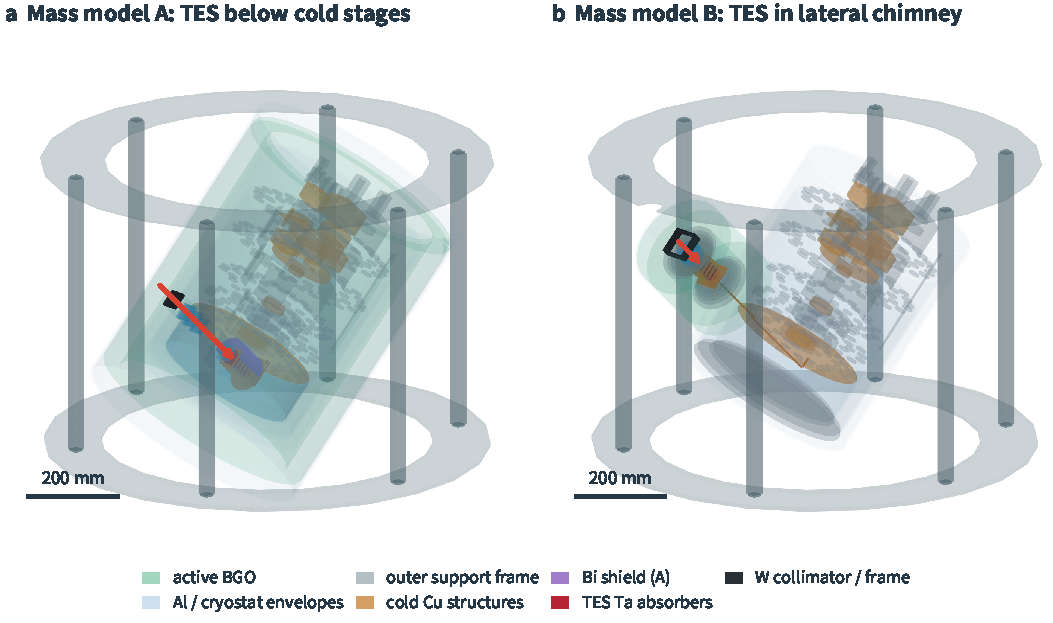
\includegraphics[width=0.98\linewidth]{figures/manuscript/fig01_mass_models_ab_en.pdf}
\caption{Matched detector--cryostat views of (a) mass model A and (b)
mass model B, rendered with the same viewing angle and scale. In model A, the
six-layer TES array lies below the staged cold structures and behind a
multihole W collimator. Model B translates the same TES core into a lateral Al
side chimney, with local active BGO on the chimney side, front optical annulus,
and rear cold-port annulus. Red arrows show the nominal focused 511 keV paths;
selected outer envelopes are translucent or omitted for clarity.}
\label{fig:mass_model}
\end{figure}

Both designs use the same MEGAlib/Geant4 framework, source fields, TES response,
timing, and selection algorithms; active channels and physical apertures are
geometry-specific.

\FloatBarrier

\section{Simulation framework}
\label{sec:framework}

Particle transport was performed with Cosima in MEGAlib 4.02.00 (Geant4
10.02.p03), using the \texttt{LivermorePol} electromagnetic and
\texttt{qgsp-bic-hp} hadronic physics lists
\cite{Zoglauer2006,Agostinelli2003,Allison2016}. Cosima defines sources and
detector geometry, transports particles through the mass model, and records
interactions for detector-response and event-selection analysis.
A uniform Geant4 production range cut of \(5\,\mu\mathrm{m}\) was used.
Figure~\ref{fig:workflow} summarizes the end-to-end
calculation in three physical branches: focused signal, prompt atmospheric
background, and delayed activation background. The Laue optics and the
detector--cryostat system were represented by separate mass models. The
reference point source was first transported through the Laue-lens model; the
positions and directions of photons reaching the focal plane were written to a
MEGAlib EventList and used to initialize detector-side Monte Carlo transport.
The focused signal and all backgrounds were transported through each
detector--cryostat mass model.

Prompt transport and activation-production transport were run in parallel from
the same eight-family EXPACS/PARMA atmospheric field, comprising
$\gamma$, $e^-$, $e^+$, $\mu^-$, $\mu^+$, $n$, $p$, and $\alpha$. In
the delayed-activation branch, BUILDUP transport recorded nuclide yields,
material volumes, and production positions. These records were used to
calculate the activity accumulated during the flight and to construct the
radionuclide inventory at each reference epoch; delayed decays were then
sampled at the recorded production positions and transported through the
detector--cryostat model.

The focused signal, eight prompt families, and delayed activation use the same
detector response within each model. The science-window cut is followed by the
geometry-specific active veto and common Compton-topology test. Selected
backgrounds are decomposed by incident particle, parent nuclide, material, and
production volume before the mission fold. The subsections below define the
source models, transport normalization, event selection, and mission-time
calculation.

\begin{landscape}
\centering
\vspace*{\fill}
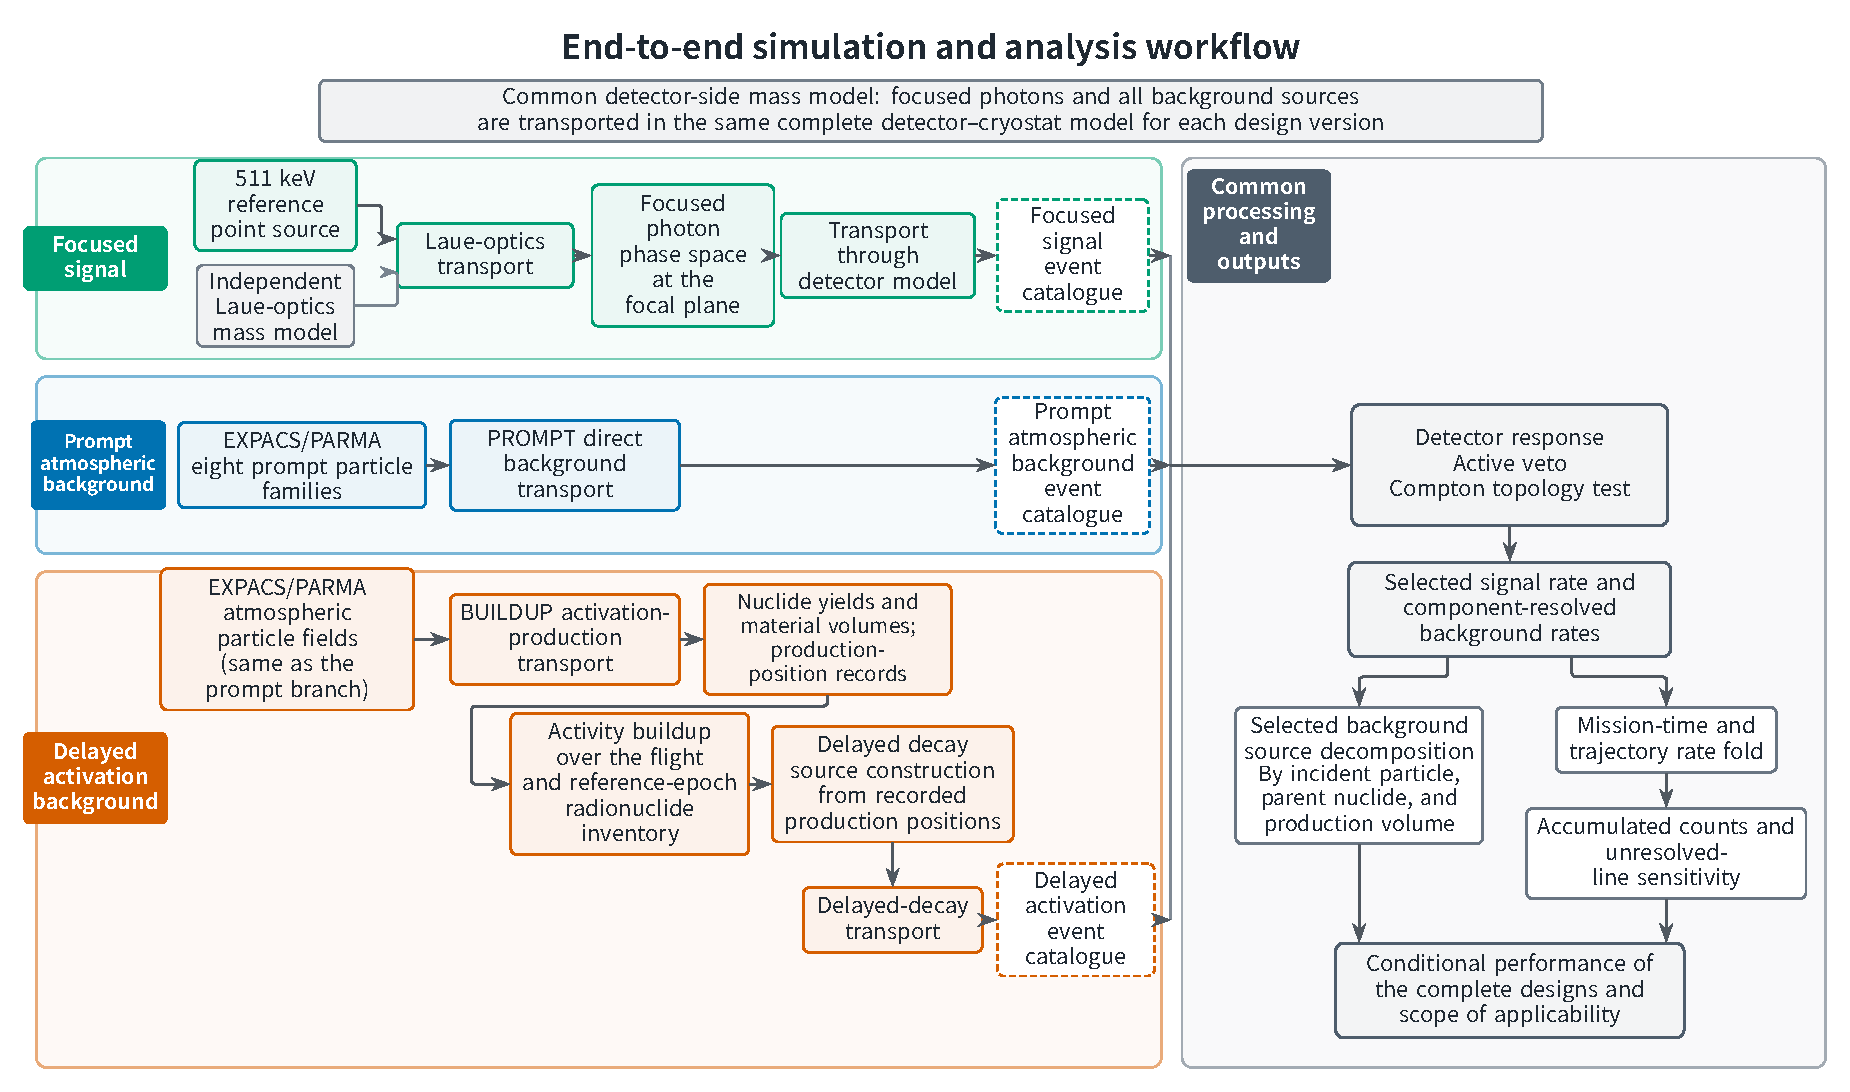
\includegraphics[width=0.97\linewidth]{figures/manuscript/fig02_workflow_en_threebranch_20260830.pdf}
\captionof{figure}{End-to-end simulation and analysis workflow. The focused
signal, prompt atmospheric background, and delayed activation form three
physical branches. The prompt branch comprises eight independently
normalized particle families ($\gamma,e^-,e^+,\mu^-,\mu^+,n,p,\alpha$). All
streams undergo the common detector response, active veto, and Compton-topology
test within each mass model. Selected-event provenance motivates model B; both
designs are then evaluated on the common
mission timeline.}
\label{fig:workflow}
\vspace*{\fill}
\end{landscape}

\FloatBarrier

\subsection{Laue optics and detector-coupled signal transport}
\label{sec:optics}

The simulated Laue lens uses mosaic Ge(111) crystals \cite{Barriere2009Laue,Barriere2011LauePrototype}. The optical design has a 10 m focal length, a single-ring reference response at 511\keV{}, and an effective area of $20.1\,\mathrm{cm^2}$ at 511\keV, calculated as
\begin{equation}
  A_{\mathrm{eff}}(E)=A_{\mathrm{inc}}\frac{N_{\mathrm{fp}}(E)}{N_{\mathrm{inc}}(E)}
  \label{eq:laue_aeff}
\end{equation}
where $A_{\mathrm{inc}}$ is the Monte Carlo incident sampling area, $N_{\mathrm{inc}}(E)$ is the number of incident photons, and $N_{\mathrm{fp}}(E)$ is the number of photons satisfying the focusing/focal-plane interception condition.
The mosaic-crystal implementation provides the specified angular acceptance and is used consistently throughout the optical transport.

Diffraction is implemented as a discrete application-layer process in Geant4 rather than as an efficiency applied after transport \cite{Agostinelli2003,Allison2016}. At angular offset $|\Delta\theta|$, the tabulated diffraction probability $R$ is first normalized to the unabsorbed fraction, $R_{\mathrm{eff}}=R/(1-A)$, where $A$ is the photoelectric-absorption probability. It is then converted to an equivalent mean free path $\lambda_{\mathrm{diff}}$ through
$1-\exp(-\ell/\lambda_{\mathrm{diff}})=R_{\mathrm{eff}}$, where $\ell$ is the photon path length through the crystal step; hence $\lambda_{\mathrm{diff}}=-\ell/\ln(1-R_{\mathrm{eff}})$. Geant4 samples this process together with photoelectric absorption and Compton scattering, and the shortest sampled interaction length determines which process occurs first. A photon not selected for diffraction therefore continues under the standard electromagnetic physics and may be absorbed, scattered, or transmitted.

In this work, the diffraction probability is determined from a precomputed XOP/CRYSTAL rocking curve. The angular dependences of the Ge(111) reflectivity, transmissivity, and absorption are generated with the CRYSTAL/diff\_pat module of the XOP toolkit (called through xoppylib using crystallographic data from DABAX) \cite{SanchezDelRio2011XOP} and stored as a transport lookup table during preprocessing. At each transport step inside a crystal, the angular deviation from the Bragg condition is evaluated and the corresponding diffraction probability is obtained by interpolation. The 30 arcsec FWHM mosaic spread is implemented by applying a Gaussian angular perturbation to the ideal Bragg-plane normal. When diffraction occurs, the outgoing direction is determined from the perturbed plane normal, while the photon energy is conserved. This treatment follows existing Geant4 implementations of crystal Bragg reflection \cite{Guan2023BraggReflection,Reiazi2025G4BraggReflection} and is applied to the energy range considered here.

Here the reference signal is a monochromatic 511\keV{} point source. Its sole
reference normalization is $\fref=2.4\times10^{-4}\phcms$ above the atmosphere
(Section~\ref{sec:requirements}), motivated by the dedicated INTEGRAL/IBIS
compact-source upper limit \cite{DeCesare2011} rather than by any single
observed object. It is constructed as a MEGAlib far-field source
\cite{Zoglauer2006}, with the detailed construction given in
Section~\ref{subsec:pointsource}. The signal is transported through the optics
branch and injected into the detector mass model as a parallel-beam source;
prompt cosmic-ray background and activation decays are transported directly in
the detector/cryostat mass model. The primary background budget is therefore
defined for the detector/cryostat branch, while the optics branch supplies the
transported focal-plane signal phase space.

\subsection{Source construction}
\label{sec:background}

The reference point-source EventList, the prompt atmospheric field, and the
delayed-decay source are constructed independently. The eight prompt
particle families retain separate physical-rate normalizations; activation production and delayed
decay remain separate transport stages. This organization preserves the
normalization and provenance needed to compare all selected background streams
under the common detector response and event selection.

\subsubsection{Prompt atmospheric source}
\label{subsec:prompt_source}

The prompt atmospheric field is derived from EXPACS/PARMA. PARMA3.0 is an
analytical model parameterized from PHITS atmospheric-shower calculations and
benchmarked against terrestrial cosmic-ray measurements, and EXPACS is its
public tabulation and software interface
\cite{Sato2015EXPACS,Sato2016PARMA4}. PHITS supplies the underlying
particle-transport physics: primary cosmic rays interact with air nuclei, the
secondary hadrons, leptons, photons, and neutrons are transported through the
atmospheric column, and the resulting fluences are parameterized by altitude,
geomagnetic cutoff, solar modulation, energy, and direction. In this work
EXPACS/PARMA provides the differential incident flux as a function of particle
species, kinetic energy, zenith angle, geographic position, altitude, cutoff
rigidity, and solar activity, and is used only to construct the external
radiation fields; detector response, vetoing, topology selection, and
mission-time counting are applied downstream. The transport templates
use latitude $34^\circ$, longitude $100^\circ$, altitude $38\,\mathrm{km}$,
vertical cutoff rigidity $R_c=11.6\,\mathrm{GV}$, and the 2025-08-31 solar
condition corresponding to $W=118.3$.

The prompt source includes photons, neutrons, electrons, positrons, protons,
alpha particles, and negative and positive muons. For each particle family the
EXPACS/PARMA differential spectrum is converted into a MEGAlib far-field area
source covering the full zenith range $\theta=0^\circ$--$180^\circ$ and full
azimuth range $\phi=0^\circ$--$360^\circ$. The zenith dependence is represented
by 20 equal-$\mu$ bins, where $\mu=\cos\theta$: the first ten are down-going and
the last ten up-going or albedo-like. Both
hemispheres are retained in the prompt transport and in the
activation-production transport, so upward albedo particles are not discarded
at source construction. Figure~\ref{fig:expacs_fullsphere_flux} shows the
resulting full-sphere flux field.

\begin{figure}[t]
\centering
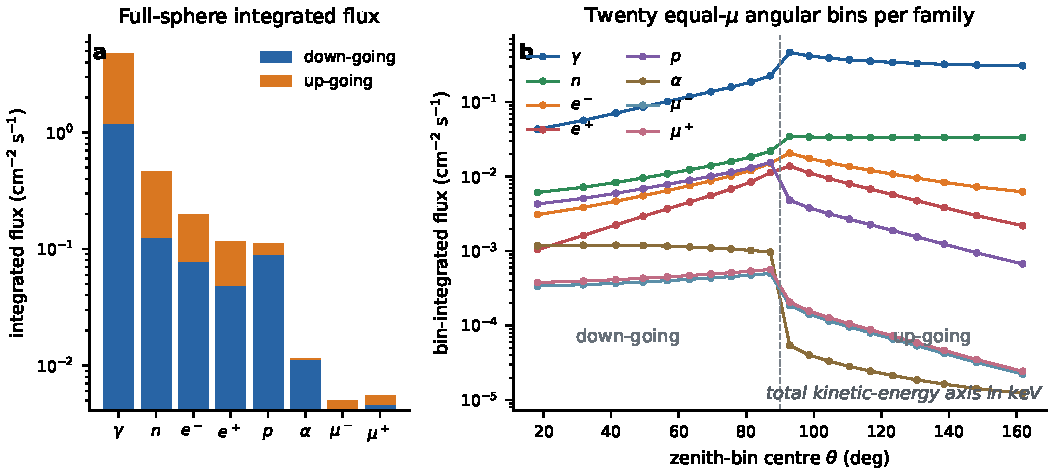
\includegraphics[width=\linewidth]{figures/manuscript/fig03_corrected_kev_sources.pdf}
\caption{EXPACS/PARMA atmospheric particle field used for prompt transport and
activation production. (a) Fluxes of the eight particle families integrated over
energy and solid angle in the down-going and up-going (albedo) hemispheres.
(b) Integrated fluxes in the 20 equal-$\mu$ zenith bins ($\mu=\cos\theta$) for
each particle family. The environment is latitude $34^\circ$, longitude
$100^\circ$, altitude $38\,\mathrm{km}$, $R_c=11.6\,\mathrm{GV}$, and $W=118.3$.}
\label{fig:expacs_fullsphere_flux}
\end{figure}

The full-sphere integrated fluxes in the adopted atmospheric tables are 4.800, 0.4622, 0.1990,
0.1170, 0.1123, 0.01149, 0.004969, and
$0.005570\,\mathrm{cm^{-2}\,s^{-1}}$ for $\gamma$, $n$, $e^-$, $e^+$, $p$,
$\alpha$, $\mu^-$, and $\mu^+$, respectively.



If $I_j(E,\mu)$ denotes the EXPACS/PARMA differential intensity for family $j$,
the flux carried by equal-$\mu$ bin $m$ is
\begin{equation}
 \Phi_{j,m}=2\pi\int_{\mu_m}^{\mu_{m+1}}\!\mathrm d\mu
             \int I_j(E,\mu)\,\mathrm dE,
 \qquad \Delta\mu=0.1,
 \label{eq:source_bin_flux}
\end{equation}
so each bin subtends $\Delta\Omega=2\pi\Delta\mu=0.6283\,\mathrm{sr}$.

All eight particle families use a far-field area source of radius
$R=60\,\mathrm{cm}$. For each sampled direction, starting positions are drawn
uniformly from the projected disk perpendicular to that direction, and momenta
point into the mass model; the geometric rate factor is the projected area
$\pi R^2$. Together, the 20 bins cover $4\pi$ incident solid angle. The same
atmospheric-field definition is used separately for prompt transport and
activation-production calculations.

\begingroup

Each accepted production job for particle family $j$
contains the complete 20-bin angular mixture; the angular bins are not treated
as independent exposures. The family source rate and the merged equivalent
exposure are therefore
\begin{equation}
 \dot N^{\mathrm{src}}_{j}=\pi R^2\sum_{m=1}^{20}\Phi_{j,m},
 \qquad
 T^{\mathrm{eq}}_{g,j}=\sum_{q\in\mathcal Q_{g,j}}\mathrm{TT}_{g,j,q}
 \simeq
 \frac{\sum_q N^{\mathrm{sim}}_{g,j,q}}{\dot N^{\mathrm{src}}_{j}},
 \qquad
 w^{\mathrm{pr}}_{g,j}=\frac{1}{T^{\mathrm{eq}}_{g,j}},
 \label{eq:prompt_equivalent_exposure}
\end{equation}
where $q$ indexes independent mergeable jobs and $\mathrm{TT}_{g,j,q}$ is the
validated physical runtime recorded in the corresponding receipt. Increasing
the number of transported primaries extends $T^{\mathrm{eq}}$ and reduces Monte
Carlo uncertainty without changing the physical source intensity.

Equation~(\ref{eq:prompt_equivalent_exposure}) applies directly to the seven
non-$\gamma$ families. Prompt atmospheric photons were transported from the
corrected-keV 20-bin broadband total spectrum and each detector-positive record
was reweighted once to the de-lined continuum as
$w_e=(T^{\mathrm{eq}}_{g,\gamma})^{-1}
J_{\mathrm{cont}}(m_e,E_e)/J_{\mathrm{total}}(m_e,E_e)$. Here
$m_e=\operatorname{clip}[\lfloor10(1+d_{z,e})\rfloor,0,19]$, and both spectra
were linearly interpolated on the same energy grid. Validation confirmed
source-flux closure and complete incident-record matching for both models.

\endgroup

\subsubsection{Delayed activation source}
\label{subsec:delayed_source}

The delayed source is built from a separate activation-production transport. It
is not counted as immediate detector background; instead, it records the isotope,
material volume, incident family, and production position of each radioactive
product. Ground-state half-lives are checked against NUBASE2020
\cite{Kondev2021NUBASE}. For isotope $k$,
\begin{equation}
  A_k(t_{\mathrm{flight}})=P_k\left[1-\exp(-\lambda_k t_{\mathrm{flight}})\right],
  \qquad \lambda_k=\frac{\ln2}{t_{1/2,k}},
\end{equation}
where $P_k$ is the production rate and the reference state is
$t_{\mathrm{flight}}=15\,\mathrm{d}$.

\begingroup

In the standard output configuration used here,
MEGAlib/Cosima's compressed \texttt{sim.gz} event files do not retain the
complete radioactive-product production information required to reconstruct
the spatial distribution of the delayed source. Because Cosima uses Geant4 as
its transport engine, we added a recording hook to \texttt{SteppingAction} to
store the production coordinate, material volume, nuclide, and excitation
state when each radioactive product was created. These fields were then used
to match the day-15 inventory to the production records and to organize the
delayed source by incident family, material category, production volume, and
coordinate.

Retaining the production positions is essential because the ability of a
delayed particle to escape the surrounding material, trigger the
geometry-specific active anticoincidence, or pass the Compton-topology
selection depends on where it was produced. Balancing computational
cost against statistical precision, we constructed $10^4$ activation-position
point sources for each incident-particle family. Sampling was weighted by the
day-15 activity of each radionuclide in its production volume, and the decay
position was drawn with equal probability from the matched simulated
production coordinates. The activation-source positions in the two mass
models, together with the parent nuclides contributing to the TES 511 keV
response window, are shown in
Fig.~\ref{fig:activation_source_positions}.
\endgroup



\begingroup

For each incident-particle family, each mass model
transports $N^{\mathrm{dec}}_{g,j}=10^6$ delayed decays. At the day-15 reference
epoch, the constant-activity equivalent exposure and per-event rate weight of
that family are
\begin{equation}
 T^{\mathrm{eq,del}}_{g,j}(t_{\mathrm{ref}})
 =\frac{N^{\mathrm{dec}}_{g,j}}{A_{g,j}(t_{\mathrm{ref}})},
 \qquad
 w^{\mathrm{del}}_{g,j}(t_{\mathrm{ref}})
 =\frac{A_{g,j}(t_{\mathrm{ref}})}{N^{\mathrm{dec}}_{g,j}}
 =\frac{1}{T^{\mathrm{eq,del}}_{g,j}(t_{\mathrm{ref}})},
 \quad t_{\mathrm{ref}}=15\,\mathrm{d}.
 \label{eq:delayed_equivalent_exposure}
\end{equation}
Here $T^{\mathrm{eq,del}}$ is the Monte Carlo equivalent sampling time for the
day-15 activity mixture, rather than the elapsed flight time or the BUILDUP
irradiation time; the mission fold updates the day-15 reference weights at each
time node using the parent-nuclide activity curves.
\endgroup

Table~\ref{tab:background_source_model} summarizes the prompt and delayed
transport statistics and their rate normalizations.

\begingroup

\begin{table}[!htbp]

\centering

\caption{Particle-family transport statistics and rate
normalization for the two mass models. $N_{\mathrm{tr}}$ and $N_{\mathrm{dec}}$
are transported prompt primaries and delayed decays, respectively;
$T_{\mathrm{eq}}$ is the summed physical exposure of accepted independent
production batches; and $N_{\mathrm{det+}}$ counts templates with a positive
raw deposit in the TES or an active shield. $R_{\mathrm{cat}}$ is the
detector-positive occupancy rate actually supplied to common-time Poisson
sampling. It is evaluated before detector-response smearing, the pixel
threshold, science window, active veto, and Compton selection. In panel (b),
$T_{\mathrm{eq,del}}=N_{\mathrm{dec}}/A_{g,j}(15\,\mathrm d)$, as defined in
Equation~(\ref{eq:delayed_equivalent_exposure}).}
\label{tab:background_source_model}
\scriptsize
\setlength{\tabcolsep}{5.0pt}
\renewcommand{\arraystretch}{0.92}
\noindent\textit{(a) Prompt atmospheric-particle transport}\par\vspace{0.20em}
\begin{tabular}{clrrrr}
\toprule
Model & Family & $N_{\mathrm{tr}}$ & $T_{\mathrm{eq}}$ (s)
& $N_{\mathrm{det+}}$ & $R_{\mathrm{cat}}$ ($\mathrm{s^{-1}}$) \\
\midrule
A & $\gamma$ & $20{,}315{,}706$ & 374.2 & $6{,}372{,}612$ & $1.636\times10^{4}$ \\
A & $n$ & $1{,}164{,}960$ & 223.1 & $403{,}599$ & $1.809\times10^{3}$ \\
A & $e^-$ & $675{,}057$ & 299.8 & $287{,}509$ & 959.1 \\
A & $e^+$ & $394{,}119$ & 298.9 & $182{,}318$ & 610.0 \\
A & $p$ & $380{,}829$ & 299.8 & $172{,}734$ & 576.3 \\
A & $\alpha$ & $39{,}050$ & 299.0 & $18{,}657$ & 62.41 \\
A & $\mu^-$ & $16{,}607$ & 298.2 & $7{,}529$ & 25.25 \\
A & $\mu^+$ & $19{,}371$ & 308.7 & $8{,}629$ & 27.96 \\
\addlinespace[0.25em]
B & $\gamma$ & $112{,}421{,}262$ & 2071 & $4{,}189{,}660$ & $1.940\times10^{3}$ \\
B & $n$ & $8{,}363{,}786$ & 1599 & $325{,}382$ & 203.4 \\
B & $e^-$ & $3{,}602{,}914$ & 1599 & $136{,}738$ & 85.52 \\
B & $e^+$ & $2{,}119{,}548$ & 1601 & $139{,}963$ & 87.42 \\
B & $p$ & $2{,}036{,}710$ & 1603 & $123{,}624$ & 77.13 \\
B & $\alpha$ & $209{,}074$ & 1608 & $18{,}285$ & 11.37 \\
B & $\mu^-$ & $91{,}020$ & 1608 & $4{,}605$ & 2.864 \\
B & $\mu^+$ & $102{,}306$ & 1613 & $5{,}268$ & 3.266 \\
\bottomrule
\end{tabular}

\vspace{0.45em}
\noindent\textit{(b) Delayed-decay transport at day 15}\par\vspace{0.20em}
\begin{tabular}{clrrrr}
\toprule
Model & Family & $N_{\mathrm{dec}}$ & $T_{\mathrm{eq,del}}$ (s)
& $N_{\mathrm{det+}}$ & $R_{\mathrm{cat},15}$ ($\mathrm{s^{-1}}$) \\
\midrule
A & $\gamma$ & $1.0\times10^6$ & $1.517\times10^5$ & $884{,}678$ & 5.832 \\
A & $n$ & $1.0\times10^6$ & 3030 & $893{,}664$ & 294.9 \\
A & $e^-$ & $1.0\times10^6$ & $1.497\times10^6$ & $853{,}592$ & 0.5701 \\
A & $e^+$ & $1.0\times10^6$ & $3.386\times10^5$ & $904{,}775$ & 2.672 \\
A & $p$ & $1.0\times10^6$ & 1381 & $916{,}824$ & 664.0 \\
A & $\alpha$ & $1.0\times10^6$ & 3478 & $918{,}773$ & 264.2 \\
A & $\mu^-$ & $1.0\times10^6$ & $4.034\times10^6$ & $871{,}246$ & 0.2160 \\
A & $\mu^+$ & $1.0\times10^6$ & $7.934\times10^{14}$ & $1{,}000{,}000$ & $1.260\times10^{-9}$ \\
\addlinespace[0.25em]
B & $\gamma$ & $1.0\times10^6$ & $4.921\times10^5$ & $396{,}106$ & 0.8049 \\
B & $n$ & $1.0\times10^6$ & $1.459\times10^4$ & $554{,}831$ & 38.02 \\
B & $e^-$ & $1.0\times10^6$ & $3.755\times10^6$ & $433{,}022$ & 0.1153 \\
B & $e^+$ & $1.0\times10^6$ & $1.481\times10^6$ & $531{,}844$ & 0.3592 \\
B & $p$ & $1.0\times10^6$ & 9476 & $694{,}056$ & 73.24 \\
B & $\alpha$ & $1.0\times10^6$ & $2.917\times10^4$ & $711{,}199$ & 24.38 \\
B & $\mu^-$ & $1.0\times10^6$ & $1.462\times10^7$ & $436{,}535$ & 0.02986 \\
B & $\mu^+$ & $1.0\times10^6$ & $2.521\times10^8$ & $1{,}867$ & $7.405\times10^{-6}$ \\
\bottomrule
\end{tabular}

\end{table}
\endgroup

\begin{figure}[p]
\centering
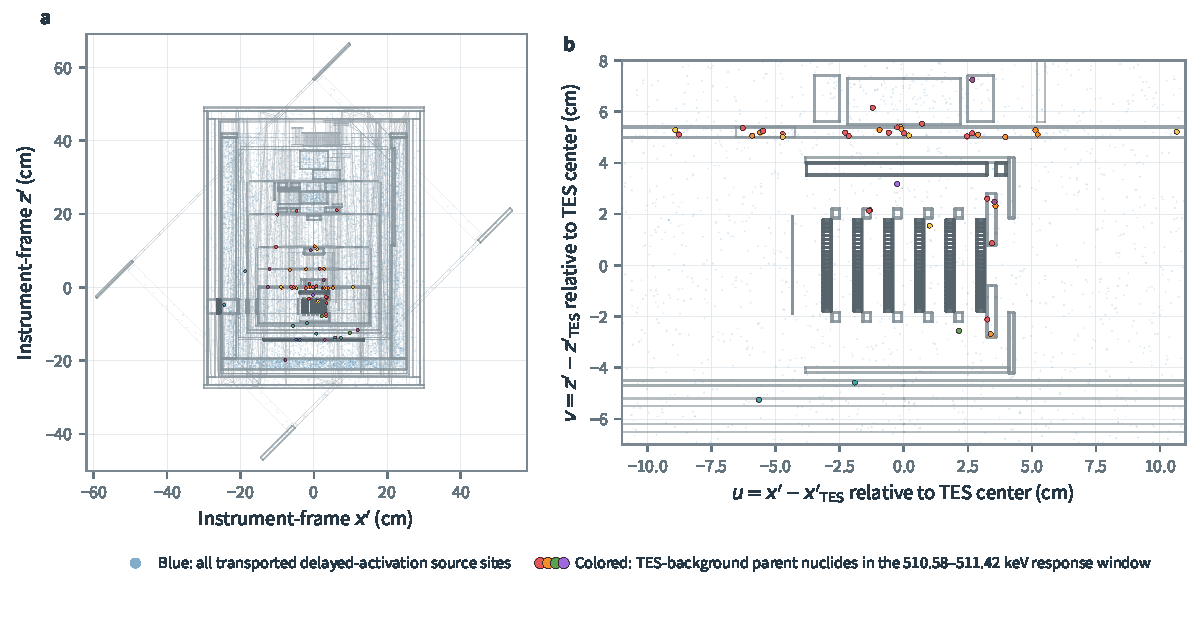
\includegraphics[width=0.96\linewidth]{figures/manuscript/fig_activation_positions_model_a_en.pdf}
\vspace{0.35em}

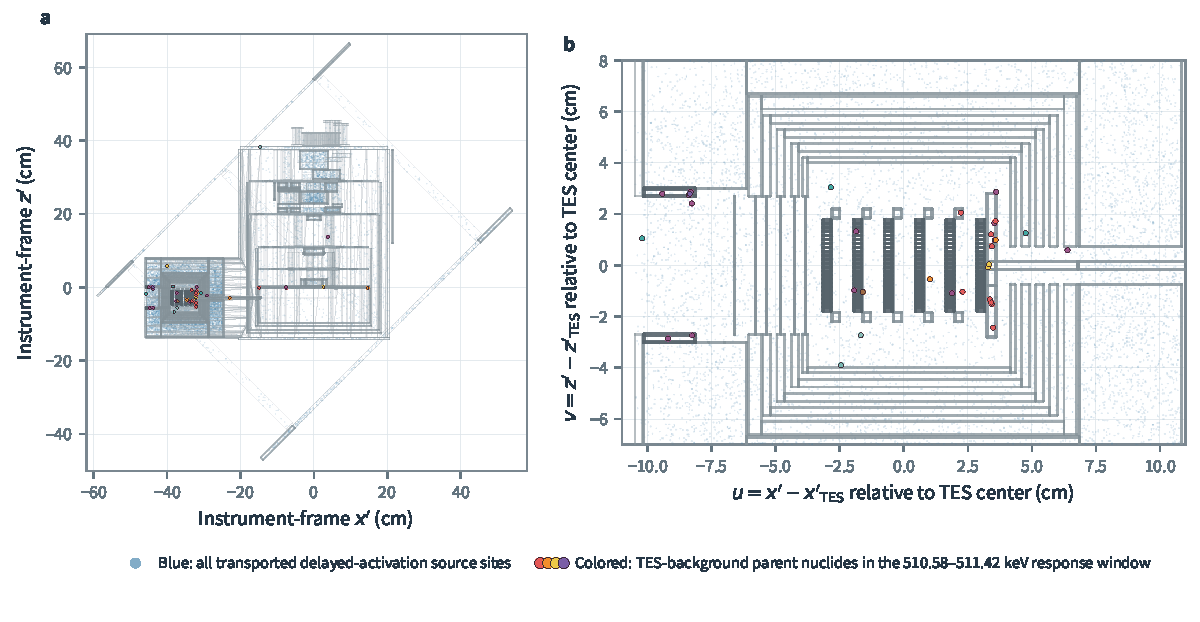
\includegraphics[width=0.96\linewidth]{figures/manuscript/fig_activation_positions_model_b_en.pdf}
\caption{Delayed activation-production positions in mass model A (top) and mass
model B (bottom). In each row, the left panel shows the full mass model and the
right panel enlarges the TES region. Blue points denote all transported delayed
activation-source positions; coloured points denote activation parent nuclides
that produce background in the TES $510.58$--$511.42$ keV response window.}
\label{fig:activation_source_positions}
\end{figure}

\FloatBarrier

\subsubsection{Reference point-source construction}
\label{subsec:pointsource}

\begingroup

The focused-signal branch uses an on-axis monochromatic 511\keV{}
far-field point source, represented by a parallel beam at the lens entrance.
The flux convention and atmospheric attenuation of the reference source are
defined in Section~\ref{sec:requirements}; this subsection specifies only the
focal-plane photon phase space and the detector effective-area calculation.

Photons are sampled uniformly over the lens aperture $A_{\mathrm{inc}}$ defined
by Equation~\eqref{eq:laue_aeff}. The 30 arcsec mosaic spread, XOP/CRYSTAL
rocking curve, and 10 m geometry set the focal-plane response. Three samples of
$1.5\times10^5$ photons yield 37,256 focal-plane crossings, of which
$N_{\mathrm{fp}}=37{,}194$ fall within the $r=1.898\,\mathrm{cm}$ beryllium
entrance. At 10 m, $r_{90}=1.03\,\mathrm{cm}$ and
$r_{99}=1.25\,\mathrm{cm}$ correspond to $3.54$ and $4.30$ arcmin. The accepted
photon phase space forms the common EventList for both mass models.

This EventList represents the optical effective area
$A_{\mathrm{fp}}\equiv A_{\mathrm{eff}}(511\keV)=20.08\,\mathrm{cm^2}$.
Each equally weighted focal-plane photon therefore carries the area weight
\begin{equation}
 a_{\mathrm{ray}}=\frac{A_{\mathrm{fp}}}{N_{\mathrm{fp}}}.
 \label{eq:focal_eventlist_area_weight}
\end{equation}
For mass model $g$, let $N_{\mathrm{sel},g}$ be the number of focal-plane
photons retained after detector transport, response convolution, science-window
selection, the geometry-specific isolated-event active-anticoincidence
criterion, and the Compton topology/aperture selection. Both models use the
same Compton reconstruction algorithm, while aperture compatibility is tested
against the physical entrance of the corresponding model. The final on-axis
isolated-event effective area is
\begin{equation}
 A_{\mathrm{eff},g}
 =\sum_{i\in\mathrm{sel},g}a_{\mathrm{ray}}
 =A_{\mathrm{fp}}\frac{N_{\mathrm{sel},g}}{N_{\mathrm{fp}}}.
 \label{eq:selected_signal_effective_area}
\end{equation}

\endgroup



\subsection{Detector response, event selection, and veto definitions}
\label{sec:selection}

The common-time calculation maps the prompt atmospheric and delayed-activation
background catalogues onto one explicit time axis before the active-veto and
Compton selections are applied. The eight prompt particle families
retain independent physical-rate normalizations. Focused-signal events are inserted as
conditional probes of accidental-coincidence loss rather than added to the
background budget.

\subsubsection{Time axis and rate normalization}
\label{subsec:time_axis}

In a stationary radiation environment, mutually independent particle events
with a constant mean arrival rate have Poisson-distributed counts in a fixed
time interval. Conditional on the event count, their arrival times are
uniformly distributed within that interval. This provides a natural temporal
representation for rate-normalized Monte Carlo catalogues: the catalogue
supplies the energy deposits, positions, and topologies, while the Poisson
process determines how often and when those events occur on the physical time
axis.

The radiation environment evolves along the balloon trajectory, but much more
slowly than the $1\,\mu\mathrm{s}$ coincidence time scale adopted in this study.
Within each trajectory node, the event streams can therefore be approximated as
independent Poisson processes with constant arrival rates. The focused signal,
prompt atmospheric background, and delayed-activation background are generated
by separate transport calculations and do not share a physical time axis,
whereas the geometry-specific active anticoincidence and Compton-topology selections depend on all
energy deposits within the same time window. Evaluating accidental coincidences
therefore requires these catalogues to be mapped onto a common time axis.

The three transported streams acquire per-record rate weights $r_{km}$ during
the source-normalization stage of Section~\ref{sec:background}, where
$k\in\{\mathrm{signal},\mathrm{prompt},\mathrm{delayed}\}$ labels the catalogue
and $m$ labels a transported record. The total rate of catalogue $k$ is
$R_k=\sum_m r_{km}$. For a reference interval of duration $T$, the number of
instances drawn from catalogue $k$ is
\begin{equation}
 N_k\sim\mathrm{Pois}(R_kT).
 \label{eq:poisson_superposition}
\end{equation}
Records are sampled with replacement with probabilities $r_{km}/R_k$ and are
assigned independent uniform times in $[0,T]$. The resulting sequence preserves
both the physical rate and the energy, direction, and detector-response
distribution of the event stream.

The three draws are merged and ordered by arrival time. Events separated by no
more than $\tau=1\,\mu\mathrm{s}$ are linked transitively into one coincidence
candidate group $c$. All energy deposits in the group are then subjected jointly
to the science-window, geometry-specific active-anticoincidence, and Compton-topology selections.
Figure~\ref{fig:poisson_time_axis_schematic} summarizes this construction.

\begin{figure}[H]
\centering
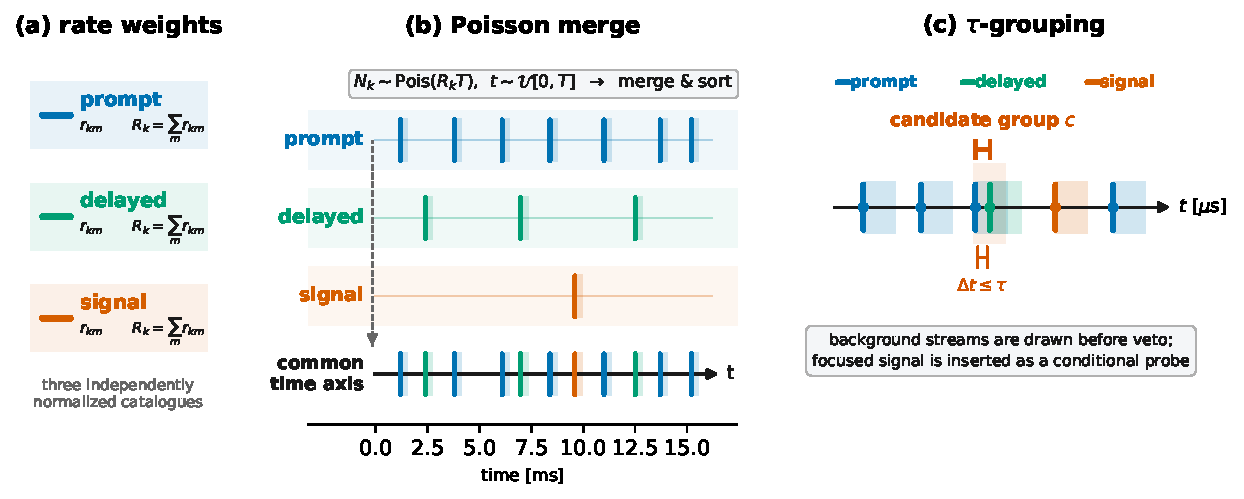
\includegraphics[width=\linewidth]{figures/manuscript/fig04a_poisson_time_axis_schematic_threebranch_20260830.pdf}
\caption{Schematic construction of the common-time coincidence axis. (a) Each
transported stream carries per-record rate weights and a total rate.
(b) Independent Poisson draws are merged and time-ordered on a common axis.
(c) Events separated by no more than $\tau=1\,\mu\mathrm{s}$ form one
coincidence candidate group. Colours identify catalogue membership; event
positions and densities are schematic. Prompt and delayed streams define the
background axis; focused signal is inserted as a conditional probe.}
\label{fig:poisson_time_axis_schematic}
\end{figure}

This calculation is performed at five reference times on days 0, 5, 10, 15,
and 20. At each reference time, the physical rates of the eight prompt
particle families and delayed activation set the
Poisson draws used to construct a common background time axis for that
reference environment. Events separated by no more than $1\,\mu\mathrm{s}$ form
one coincidence group and jointly undergo the science-window, geometry-specific
active-anticoincidence, and Compton-topology selections. Focused-signal events are
also inserted individually into the corresponding background axis to quantify
signal loss from accidental coincidences.

Instrument performance is then evaluated along the long-duration balloon
trajectory, with the 20 d flight divided into 6 h intervals. Particle fluxes,
atmospheric transmission of the signal, and the activation inventory evolve with flight
time and position, thereby changing both the event density on the common time
axis and the accidental-coincidence probability. The background corrections
and signal-survival fractions obtained at the five reference times are applied
along the full trajectory. Section~\ref{sec:mission_time_fold} specifies the
trajectory model, temporal interpolation, and cumulative-count calculation.

\subsubsection{Detector response, science window, and weighted rates}
\label{subsec:detector_response}

Before the science-window and anticoincidence decisions, TES energy deposits in
each candidate group are combined by pixel. Multiple deposits in the same pixel
are summed to give its true deposited energy, and their energy-weighted position
represents the interaction location. The expected single-pixel energy resolution
is $\Delta E_{\mathrm{FWHM}}=420\,\mathrm{eV}$; TES measurement fluctuations are
approximated by a Gaussian response with this FWHM. Pixel hits with measured
energies below $0.300\keV$ are removed. Mass models A and B use the same response
and threshold settings.

The measured energies of all retained TES pixel hits are summed to give the total
measured TES energy of the event, which is used for the 511\,keV science-window
selection. The energy, position, layer, and multiplicity of each pixel hit remain
available for the subsequent Compton-topology selection. BGO deposits are
accumulated separately, are not included in the TES total, and enter the active
anticoincidence decision in the next subsection.

The common science window has a fixed one-FWHM half-width:
$510.58\leq E_{\mathrm{TES}}<511.42\keV$ for the focused signal and all
backgrounds.



The source catalogues have different physical fluxes, transport exposures, and
source-level reweighting. Each event therefore carries a physical-rate weight,
and the signal or background rate at a given selection stage is obtained by
summing the weights of events that pass that stage. Raw record counts quantify
Monte Carlo transport support rather than physical rate. Finite-transport
statistical uncertainties are propagated from the actual weight distribution,
while focused-signal acceptance is treated binomially using the common focal-plane
sample. Long-duration rate propagation along the mission trajectory is described
in Section~\ref{sec:mission_time_fold}; the response-convolved spectra through
the active-veto and topology/aperture stages are reported with the cut-flow results.

\subsubsection{Active anticoincidence gate}

Active anticoincidence rejects events that produce a 511\,keV candidate in the
TES while also depositing energy in the surrounding active shield. Passive
shielding attenuates incident radiation, whereas active BGO provides
time-coincident information for event-by-event discrimination. A focused
511\,keV photon reaches the TES mainly through the optical channel. Atmospheric
charged particles, secondaries from hadronic interactions, and some
high-energy atmospheric-$\gamma$ cascades are more likely to deposit energy in both the TES
and the surrounding active volumes. Coincident BGO energy can therefore
identify background candidates in the science window.

The active gate uses the common time axis and $1\,\mu\mathrm{s}$ coincidence
groups defined in Section~\ref{subsec:time_axis}. Within each candidate group,
TES deposits are first combined by pixel and then passed through the response
defined in Section~\ref{subsec:detector_response}; the science-window decision
uses the sum of the measured energies of all retained pixels. Simulated energy
deposits in all BGO volumes in the same group are summed as
$E_{\mathrm{BGO}}$. This active-volume sum is used only for anticoincidence and
does not contribute to the TES event energy.

The active system of mass model A comprises a BGO side shell, bottom cap, and
top annulus. The active system of mass model B comprises the chimney side
shield, front optical annulus, and rear cold-port annulus. Both mass models use
the same group-level passing condition,
\[
 E_{\mathrm{BGO}}<50\keV .
\]
The common offline threshold is applied to the group-summed BGO deposit;
$E_{\mathrm{BGO}}\geq50\keV$ vetoes the group.
Within a given mass model, the same group-level criteria are applied to the
focused signal, eight-family prompt background and delayed
activation.

The groupwise sums include both correlated TES--shield deposits from one
incident particle and accidental overlap of otherwise independent hits whose
arrival times satisfy the $1\,\mu\mathrm{s}$ linking rule. A focused photon can
therefore be rejected when an unrelated active-shield hit enters the same
coincidence group. The associated loss is described by the accidental
signal-survival fraction defined in Section~\ref{subsec:time_axis} and included
in the mission-time fold. Candidates that pass the active gate proceed to the
Compton-topology and entrance-aperture consistency selection.

\subsubsection{Compton topology and entrance-aperture consistency}

Active anticoincidence removes candidates with energy deposits above the adopted
threshold in the surrounding scintillators, but it cannot distinguish a focused photon from a
background event whose interactions remain within the TES array. Either can
leave a total energy near 511\,keV in the focal plane. A focused photon must,
however, arrive through the side-entry optical channel. For an event with two
or more separated TES hits, the division of energy among the hits and their
relative positions constrain the possible arrival directions. We therefore test
whether each event is compatible with the entrance aperture. The test uses the
kinematic cone construction of a Compton camera
\cite{Zoglauer2006}, but only as an aperture-consistency veto, not for imaging
or source localization.

The six-layer pixelated TES focal plane provides the information needed for
this test at pixel scale. For the retained hits defined in
Section~\ref{subsec:detector_response}, the response model supplies a measured
energy, while the event catalogue preserves the TES layer and pixel position.
Hits in different pixels or layers therefore provide both an energy division
and a finite spatial lever arm. The catalogue does not determine the interaction
order or the position within a pixel. A single-hit event consequently carries
no Compton-direction information and is retained as a calorimetric line
candidate; multi-hit events proceed to the consistency test below.

For an assumed interaction order, let a candidate of total energy $E_0$ deposit
$E_1$ at the first representative position $\mathbf r_1$ and then propagate
with $E_{\mathrm{sc}}=E_0-E_1$ to a second position $\mathbf r_2$. The measured
energies give the Compton scattering angle
\begin{equation}
  \cos\theta_C =
  1 - m_ec^2\left(\frac{1}{E_{\mathrm{sc}}}
  - \frac{1}{E_1+E_{\mathrm{sc}}}\right).
\end{equation}
The vector $\mathbf r_2-\mathbf r_1$ fixes the scattered-photon direction
$\hat{\mathbf u}_{12}$, but not the incident direction. Together,
$\hat{\mathbf u}_{12}$ and $\theta_C$ define a cone of allowed incident
directions with apex $\mathbf r_1$ and axis $-\hat{\mathbf u}_{12}$. The event
is aperture compatible if this cone intersects a circular analysis disk in the
side-entry plane. The disk radii are $1.898\,\mathrm{cm}$ for mass model A and
$1.900\,\mathrm{cm}$ for mass model B. These disks define the geometric region
used by the selection; they are not the complete physical windows or collimator
openings.

The remaining position uncertainty is handled explicitly. The catalogue gives
an analysis position for each hit, but does not resolve the interaction point
within the pixel. We represent that uncertainty by an axis-aligned box centred
on the recorded position, with half-lengths $0.075$, $0.075$, and
$0.150\,\mathrm{cm}$ along the analysis $x$, $y$, and $z$ axes. Its eight
vertices and centre give nine representative positions, not nine additional
measurements. For an assumed order of the first two hits, the two boxes produce
$9\times9=81$ position pairs and hence 81 candidate cones. Each cone is sampled
at 24 uniformly spaced azimuths and extended forward to the entrance plane. The
cone intersects the disk if a sampled point lies inside it or if a segment
joining adjacent samples crosses it. The test is deliberately permissive: one
intersection among the 81 candidate cones is enough to retain that order.
Figure~\ref{fig:compton_aperture_consistency} summarizes this construction.

\begin{figure}[H]
\centering
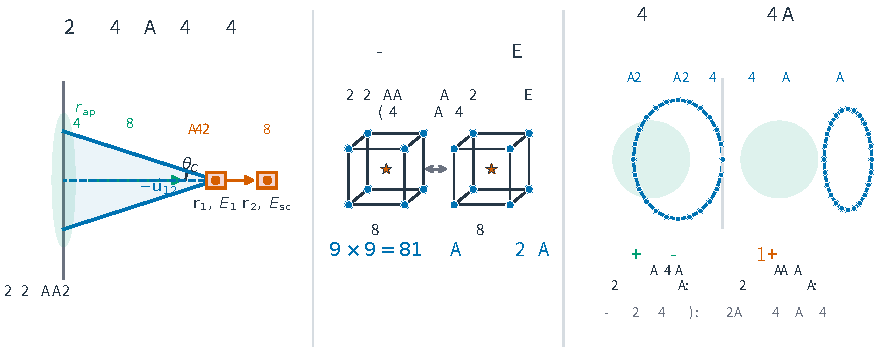
\includegraphics[width=\linewidth]{figures/fig_compton_aperture_consistency_en.pdf}
\caption{Schematic of the Compton-cone/aperture-consistency veto. (a) The first
two TES hits define a reconstruction cone from their measured energies and
representative positions; the cone is a set of allowed source directions, not a
unique photon trajectory. (b) Each hit is represented by the eight vertices and
centre of an axis-aligned analysis box, giving $9\times9=81$ position hypotheses
for a specified order. (c) The cone trace in the entrance plane is approximated
by 24 azimuthal samples and their connecting segments. An intersection with the
analysis-aperture disk retains the event, whereas a valid reconstruction that
misses the disk is vetoed. Events without a valid cone remain in the rate
accounting as unreconstructed. The schematic is not to scale.}
\label{fig:compton_aperture_consistency}
\end{figure}

The interaction order is treated separately from the within-pixel position
uncertainty. For a two-hit event, both orders are tested and either compatible
order is sufficient. For an event with at least three hits, all orders are first
enumerated using the recorded analysis positions. For a candidate sequence of
$n$ hits $\{(\mathbf r_j,\epsilon_j)\}_{j=1}^{n}$, the Compton sequence residual
is
\begin{equation}
 Q=\sum_{i=2}^{n-1}\left(\cos\theta_{C,i}-
 \hat{\mathbf u}_{i-1,i}\!\cdot\!\hat{\mathbf u}_{i,i+1}\right)^2,
\end{equation}
where $\theta_{C,i}$ is calculated from the energy $\epsilon_i$ deposited at
hit $i$ and the remaining energy $\sum_{k=i+1}^{n}\epsilon_k$; the two unit
vectors describe the adjacent flight segments. Orders without a physical
Compton solution do not enter the ranking. We select the order with the smallest
$Q$; if two orders are tied, we choose the one with the longer first lever arm.
Only the first-scatter cone of this selected order receives the 81-position
aperture test.

The final decision is conservative. A reconstructable multi-hit event is vetoed
only when the cone or cones tested under the applicable ordering rule miss the
analysis aperture. If no candidate order has a physically valid solution, the
event is marked as unreconstructed and retained in the final rate rather than
rejected. In this way, failure to reconstruct an event is not itself treated as
evidence that the event is background.

The veto efficiency obtained with the present Compton-trajectory analysis should be regarded as a conservative lower bound. Offline analysis may achieve higher veto efficiency by optimizing the trade-off between signal retention and background rejection. Increasing the spacing between adjacent TES layers would lengthen the Compton-reconstruction lever arm of multilayer events and could further improve veto efficiency.

\subsection{From the day-15 reference result to mission-time evolution}
\label{sec:mission_time_fold}

Detector transport supplies component-response templates at 38 km. The mission
fold holds these responses fixed while propagating the focused signal, eight
prompt families, and delayed activation over the evolving environment and
inventory \cite{Gallego2025Balloon,Kierans2017}.

The synthetic reference trajectory spans 0--20 d in 81 nodes separated by
0.25 d. Its altitude ranges from 36.25 to 41.25 km, its latitude from
$33.75^\circ$ to $34.25^\circ$ N, and its longitude from $99.75^\circ$ to
$100.25^\circ$ E. At day 15, the reference state is 38.75 km,
$34^\circ$ N, and $100^\circ$ E. At $34^\circ$ N, the Galactic center
culminates at $27^\circ$, giving the minimum line-of-sight atmospheric column
toward the source. Altitude changes affect both the incident
particle field and the atmospheric transmission at 511\,keV; latitude and
longitude provide a controlled geomagnetic modulation. The trajectory provides
the same 20 d on-source exposure for both mass models; source visibility,
Earth occultation, and repointing are not folded.

For a specified top-of-atmosphere 511\,keV line flux, the focused-signal rate
away from day 15 is scaled by the atmospheric transmission,
\begin{equation}
 S^{\mathrm{dir}}_g(t)
 =S^{\mathrm{dir}}_g(t_{15})
 \frac{T_{\mathrm{atm},511}(t)}{T_{\mathrm{atm},511}(t_{15})}
 =F_{\mathrm{TOA},511}A_{\mathrm{eff},g}T_{\mathrm{atm},511}(t),
 \label{eq:mission_signal}
\end{equation}
where $g$ denotes the mass model and $A_{\mathrm{eff},g}$ includes the detector
response and the single-event acceptance of the active anticoincidence and
Compton topology/aperture selections. In the plane-parallel approximation,
$T_{\mathrm{atm},511}(t)=\exp[-\mu_{\mathrm{air}}X(t)/\sin\epsilon]$. The
day-15 vertical residual column is $3.461\,\mathrm{g\,cm^{-2}}$; with
$\epsilon=27^\circ$ and an effective dry-air mass attenuation coefficient of
$0.08736\,\mathrm{cm^2\,g^{-1}}$ \cite{NISTXCOM}, this gives
$T_{\mathrm{atm},511}(t_{15})=0.514$. The fold recalculates this transmission
at every trajectory node.

Prompt background is scaled separately for each incident family $a$,
\begin{equation}
 R_{\mathrm{prompt},g,a}(t)
 =R_{\mathrm{prompt},g,a}(t_{15})
 \frac{\Phi_a(t)}{\Phi_a(t_{15})}
 =\Phi_a(t)K_{g,a},
 \label{eq:prompt_source_response}
\end{equation}
where $\Phi_a(t)$ is the node flux and $K_{g,a}$ is the selected response
coefficient of the transport template. The within-family energy and angular
templates remain fixed; full transport is not repeated at the 81 nodes.

Delayed activation cannot be obtained by multiplying the total day-15 delayed
rate by one scale because the retained nuclides have different production
histories and half-lives. The production rate of source-parent $k$ from family
$a$ is
\begin{equation}
 P_{g,a,k}(t)
 =P_{g,a,k}(t_{15})\frac{\Phi_a(t)}{\Phi_a(t_{15})}
 =\Phi_a(t)Y_{g,a,k},
 \label{eq:activation_production}
\end{equation}
where $Y_{g,a,k}$ is fixed by the mass-model-specific production catalogue.
The production rate is interpolated linearly between adjacent nodes and
convolved exactly with radioactive decay,
\begin{equation}
 \begin{aligned}
 N_{g,a,k}(t_{\ell+1})={}&N_{g,a,k}(t_\ell)e^{-\lambda_k\Delta t_\ell}\\
 &+\int_0^{\Delta t_\ell}P_{g,a,k}(t_\ell+u)
 e^{-\lambda_k(\Delta t_\ell-u)}\,\mathrm du,\\
 A_{g,a,k}(t_\ell)={}&\lambda_kN_{g,a,k}(t_\ell).
 \end{aligned}
 \label{eq:delayed_inventory}
\end{equation}
The selected delayed rate is
\begin{equation}
 R_{\mathrm{delayed},g}(t)=
 \sum_a\sum_k A_{g,a,k}(t)\varepsilon_{g,a,k}.
 \label{eq:delayed_selected}
\end{equation}
Advancing each family--parent component preserves its half-life and selected
decay response. The initial condition is $N_{g,a,k}(0)=0$, so the calculation
does not include ground pre-activation or inventory accumulated during ascent
before the first trajectory node.

The total direct background before cross-event grouping is
\begin{equation}
 B^{\mathrm{dir}}_g(t)
 =\sum_aR_{\mathrm{prompt},g,a}(t)+R_{\mathrm{delayed},g}(t).
 \label{eq:direct_background_time}
\end{equation}
Accidental coincidence between physical streams is evaluated at common-time
anchors on days 0, 5, 10, 15, and 20. At each anchor, Poisson arrival times are
generated from the component rates and merged onto one time axis before the
$1\,\mu\mathrm{s}$ grouping, detector response, active anticoincidence, and
Compton topology/aperture selections. The calculation defines a background
correction and a focused-signal survival fraction,
\begin{equation}
 \widehat\rho_{g,r}=
 \frac{n^{\mathrm{tl}}_{g,r}/T^{\mathrm{rep}}_{g,r}}
 {B^{\mathrm{dir}}_g(t_r)},\qquad
 \widehat\eta_{g,r}=
 \frac{n^{\mathrm{pass}}_{g,r}}{N^{\mathrm{probe}}_{g,r}}.
 \label{eq:anchor_time_factors}
\end{equation}
$\widehat\rho$ converts the direct background to the final common-time rate.
It can be slightly larger than unity when accidental energy summation moves an
event into the science window and is therefore not a survival probability.
$\widehat\eta$ is the conditional survival fraction of a weak focused event.
The two factors are interpolated separately between adjacent anchors. The
equivalent exposure per anchor is $2\times10^4$ s for mass model A and
$2\times10^5$ s for mass model B.

Figure~\ref{fig:common_time_anchors} checks the event-time layer against the
uncorrected analytic fold before applying $\rho_g(t)$. For each mass model, a
separate Poisson replay is generated on days 0, 5, 10, 15, and 20 and passed
through the common-time grouping and event selections. The replay rates are
then compared with $B_g^{\mathrm{dir}}(t)$ from
Equation~\eqref{eq:direct_background_time}, evaluated on all 81 nodes. The
largest replay-only differences are $1.67\sigma$ for mass model A and
$1.09\sigma$ for mass model B; no anchor differs from the analytic direct-rate
curve by $2\sigma$. This agreement supports use of the analytic fold as the
time-dependent rate baseline within the sampled trajectory. Each replay uses
component rates from
Equations~\eqref{eq:prompt_source_response}--\eqref{eq:delayed_selected} and is
not an independent transport.

\begin{figure}[!ht]
\centering
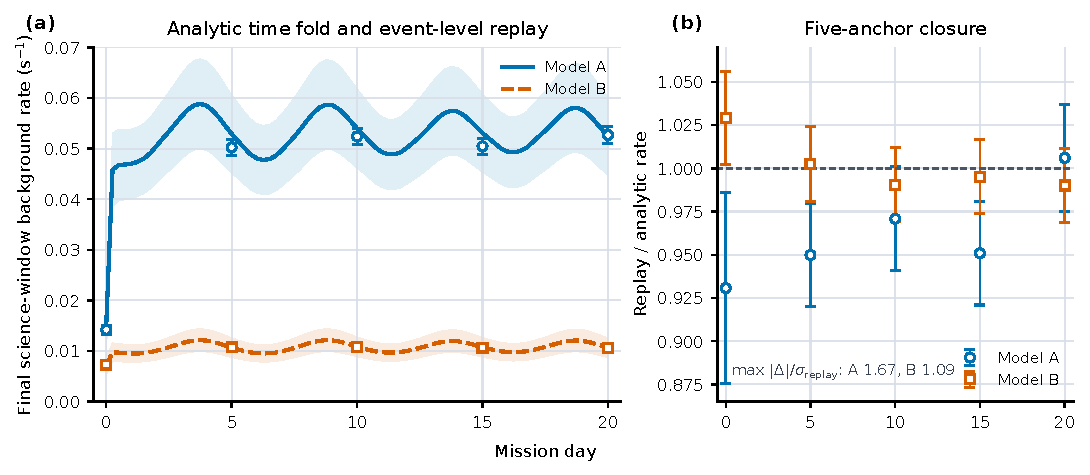
\includegraphics[width=\linewidth]{figures/section4_current/fig04_time_fold_validation.pdf}
\caption{Event-level closure of the mission-time background fold. (a) The
solid and dashed curves are the 81-node analytic direct science-window
background rates obtained from the day-15 component responses, family-resolved
environmental scaling, and nuclide-resolved activation evolution. Shaded bands
show the finite-transport $1\sigma$ template uncertainties; because the same
transport templates are reused at all nodes, these uncertainties are
correlated in time. Open symbols show separate common-time Poisson replays on
days 0, 5, 10, 15, and 20. Their error bars are $\sqrt{n}/T$, with
$T=2\times10^4$ s for mass model A and $2\times10^5$ s for mass model B.
(b) Replay-to-analytic rate ratios with replay-only statistical errors; the
horizontal line marks unity. The transport bands and replay errors are shown
separately and are not combined. Replays test rate mapping, common-time
grouping, and selection for supplied component rates; they are not independent
transports.}
\label{fig:common_time_anchors}
\end{figure}

The final time-dependent rates are
\begin{equation}
 S_g(t)=S^{\mathrm{dir}}_g(t)\eta_g(t),\qquad
 B_g(t)=B^{\mathrm{dir}}_g(t)\rho_g(t).
 \label{eq:final_time_rates}
\end{equation}
Trapezoidal integration over the 81 nodes then gives the cumulative counts at
exposure $T_n$,
\begin{equation}
 \begin{aligned}
 N_s(T_n)&=\sum_{\ell=1}^{n}\frac{S^{\mathrm{dir}}_g(t_{\ell-1})\eta_g(t_{\ell-1})+S^{\mathrm{dir}}_g(t_\ell)\eta_g(t_\ell)}{2}\,\Delta t_\ell,\\
 N_b(T_n)&=\sum_{\ell=1}^{n}\frac{B^{\mathrm{dir}}_g(t_{\ell-1})\rho_g(t_{\ell-1})+B^{\mathrm{dir}}_g(t_\ell)\rho_g(t_\ell)}{2}\,\Delta t_\ell.
 \end{aligned}
 \label{eq:cumulative_counts}
\end{equation}
The resulting $N_s(T)$ and $N_b(T)$ are the inputs to the sensitivity definition
in the next subsection. Their cumulative realization is reported in
Section~\ref{subsec:mission_fold_validation}.

\subsection{Mission significance and minimum resolvable line flux}
\label{sec:mission_sensitivity}

For cumulative signal and background counts, we define the counting
significance as
\begin{equation}
 Z(T)=\frac{N_s(T)}{\sqrt{N_b(T)}}.
 \label{eq:mission_significance}
\end{equation}
Under the high-count, weak-signal conditions considered here, this is the
large-sample limit of the Poisson counting likelihood for $N_s\ll N_b$
\cite{Cowan2011}.

The focused-signal count is linear in line flux, whereas the predicted
background is independent of a weak source. The $q\sigma$ minimum resolvable
top-of-atmosphere line flux at exposure $T$ is therefore
\begin{equation}
 F_{q\sigma}(T)=\fref\frac{q}{Z(T;\fref)},
 \qquad q\in\{3,5\}.
 \label{eq:minimum_flux}
\end{equation}
The time required to reach a specified significance is the first crossing of
$Z(T)=q$.

The same transport events are reused at all 81 mission nodes, so their
statistical errors are correlated across time. We first accumulate each event's
weighted contribution over all nodes and then calculate the statistical
uncertainty of the mission-integrated counts. Statistical errors from the five
time anchors, effective area, and signal probes are propagated into the time
curves and flux threshold. Threshold-crossing times are linearly interpolated
between adjacent nodes.

\section{Results}
\label{sec:results}

We first trace model-A backgrounds to their physical origins, then compare model
B on the common mission time axis. Both models use the response and selection
pipeline defined above, with geometry-specific active channels. For
presentation, the prompt branch is separated into atmospheric $\gamma$ rays and
the seven non-$\gamma$ families. Rates are sums of event weights, and the
common-time replay draws Poisson arrivals from those component rates.

\subsection{Baseline background and selection performance of mass model A}
\label{subsec:model_a_baseline}

Mass model A defines the reference performance. Table~\ref{tab:phase2_cutflow} gives the day-15 direct, no-coincidence cut flow in the $[510.58,511.42)\keV$ science window. The active-BGO gate reduces the total background from 3,086 records and $5.436\cps$ to 443 records and $6.071\times10^{-2}\cps$, removing 98.88\% of the pre-veto rate. The seven non-$\gamma$ prompt particle families fall from $2.912\cps$ to a zero central value, the atmospheric-$\gamma$ component falls from $2.357\cps$ to $1.789\times10^{-2}\cps$, and delayed activation falls from $0.1675\cps$ to $4.282\times10^{-2}\cps$.

After the Compton topology/aperture selection, 400 background records remain at $5.306\times10^{-2}\cps$, or 87.39\% of the active-veto rate. All 28,612 isolated focused-signal records in the measured window pass the active gate, and 28,006 survive the final selection. The corresponding effective area is $15.123\pm0.045\,\mathrm{cm^2}$, equal to 97.88\% of the measured-window signal area. Active anticoincidence supplies most of the rate reduction, while the topology selection removes a smaller residual and retains most of the focused signal.

\begin{table}[H]
\centering
\caption{Mass model A science-window cut flow. Background entries are day-15 direct, no-coincidence record counts and rates; signal entries give record counts and effective area for the common 37,194-photon focal-plane sample.}
\label{tab:phase2_cutflow}
\footnotesize
\begin{tabular}{lccc}
\toprule
Stream & Pre-veto & After active veto & Final topology/aperture \\
\midrule
Seven non-$\gamma$ prompt particle families & 869 / $2.912\cps$ & 0 / 0 & 0 / 0 \\
Atmospheric $\gamma$ & 922 / $2.357\cps$ & 7 / $1.789\times10^{-2}\cps$ & 6 / $1.534\times10^{-2}\cps$ \\
Delayed activation & 1295 / $0.1675\cps$ & 436 / $4.282\times10^{-2}\cps$ & 394 / $3.772\times10^{-2}\cps$ \\
Total background & 3086 / $5.436\cps$ & 443 / $6.071\times10^{-2}\cps$ & 400 / $5.306\times10^{-2}\cps$ \\
Focused signal & 28612 / $15.45\,\mathrm{cm^2}$ & 28612 / $15.45\,\mathrm{cm^2}$ & 28006 / $15.123\,\mathrm{cm^2}$ \\
\bottomrule
\end{tabular}
\end{table}

The nonzero components of the final direct background are delayed activation
and atmospheric $\gamma$ rays
(Table~\ref{tab:reference_background_budget}). Delayed activation contributes
$3.772\times10^{-2}\cps$ (71.10\%), and the atmospheric-$\gamma$ component contributes
$1.534\times10^{-2}\cps$ (28.91\%). Because the event weights differ among
components, record count alone does not measure statistical support; the
400-record total has $N_{\mathrm{eff}}=46.77$.

\begin{table}[H]
\centering
\caption{Day-15 final direct background of mass model A. Standard errors and effective sample sizes are calculated from $\sum_i w_i^2$ for unequal event weights.}
\label{tab:reference_background_budget}
\footnotesize
\begin{tabular}{lrrrrr}
\toprule
Component & Records & Rate / $\cps$ & Standard error / $\cps$ & $N_{\mathrm{eff}}$ & Total / \% \\
\midrule
Delayed activation & 394 & $3.772\times10^{-2}$ & $4.582\times10^{-3}$ & 67.79 & 71.10 \\
Atmospheric $\gamma$ & 6 & $1.534\times10^{-2}$ & $6.261\times10^{-3}$ & 6.00 & 28.91 \\
\midrule
Total & 400 & $5.306\times10^{-2}$ & $7.758\times10^{-3}$ & 46.77 & 100.0 \\
\bottomrule
\end{tabular}
\end{table}

\subsection{Background origins and spatial coupling in mass model A}
\label{subsec:mass_model_a_origins}



\begingroup

The preceding subsection establishes the background level of mass model A. To identify its physical origins, we traced all final events by initiating particle family. The delayed-activation component was further decomposed by parent-production material, source-volume/parent-nuclide pair, and spatial region relative to the TES.

Proton-induced activation is the largest single contribution, with 35 records and $2.485\times10^{-2}\cps$, or 46.83\% of the total direct background. The remaining delayed terms are $7.492\times10^{-3}\cps$ from $\alpha$-induced activation, $3.601\times10^{-3}\cps$ from neutron-induced activation, $1.686\times10^{-3}\cps$ from $\gamma$-induced activation, $7.021\times10^{-5}\cps$ from $e^+$-induced activation, and $2.528\times10^{-5}\cps$ from $e^-$-induced activation. Together they reproduce the final delayed rate of $3.772\times10^{-2}\cps$.

In the material decomposition, copper accounts for 70.87\% of the final delayed rate. The three leading source-volume/nuclide pairs are $^{62}$Cu produced in the TES substrate-support copper panel, the 50 mK mixing-chamber copper cold plate, and the TES-stack copper heat-sink ring. They are followed by $^{199}$Po produced in the Bi passive-shield layer and $^{64}$Cu produced in the same 50 mK cold plate and TES substrate-support copper panel. This ordering includes particle transport, detector response, active anticoincidence, and Compton selection.

Grouping the parent-production sites by transport component identifies the 50 mK mixing-chamber copper cold plate as the largest source, at 28.59\% of the final delayed rate. The two TES substrate-support copper panels (L2 and L4) contribute 27.73\%, followed by the TES-stack copper heat-sink ring at 10.18\% and the near-field Bi passive-shield layer at 7.49\%. Aluminium cryostat and shield components contribute 15.35\% in total; the remaining dilution-refrigerator/cold-stage hardware, the tungsten detector-bay bottom plate, and the BPE plus residual BGO shielding contribute 5.26\%, 3.51\%, and 1.90\%, respectively. An independent spatial projection assigns 32.18\% of the delayed rate to the DR mixing chamber and staged cold region.

Figure~\ref{fig:activation_origin_donuts} projects the same final selected delayed-activation events onto their parent-production components and initiating primary-particle families. The component projection resolves the cold plate, TES supports, and heat sink, while the particle-family projection identifies protons and $\alpha$ particles as the main drivers of this component.

\begin{figure}[!ht]
\centering
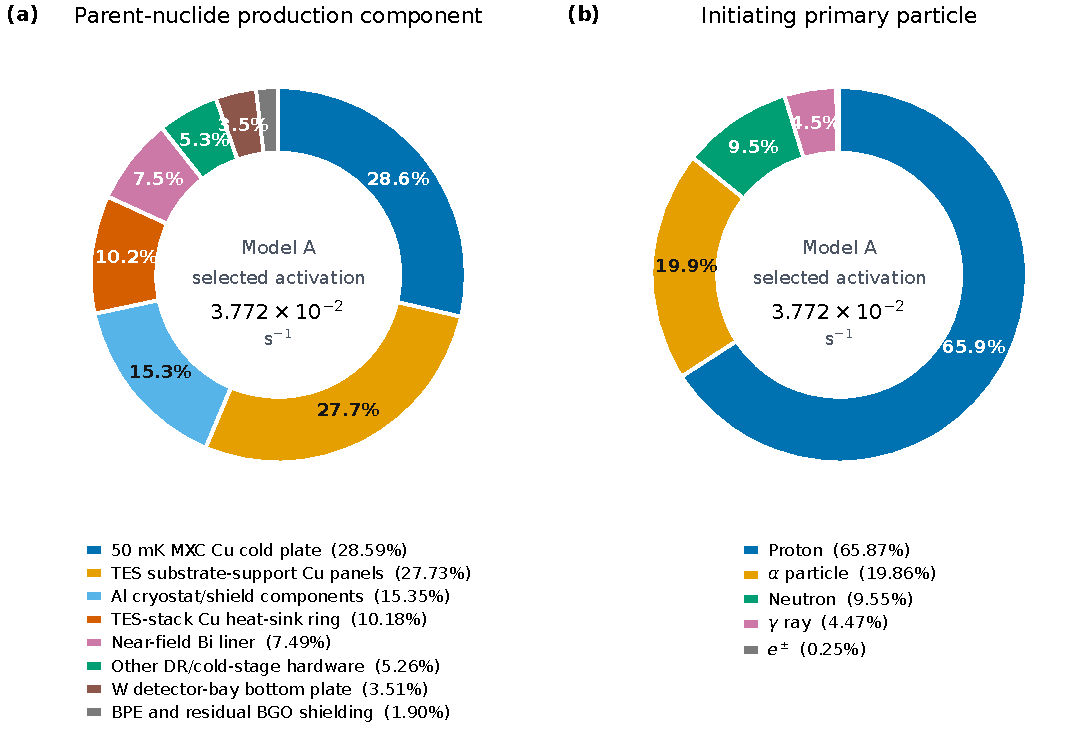
\includegraphics[width=0.96\linewidth]{figures/section4_current/fig_activation_origin_donuts_model_a.pdf}
\caption{Origins of the final selected day-15 delayed-activation background in mass model A. (a) Component in which the parent nuclide was produced. The TES substrate-support copper category combines the L2 and L4 panels; the aluminium cryostat/shield category combines the temperature-stage shield caps, inner shield cylinder, vacuum-jacket cap, and 50 mK aluminium-can bottom cap; ``other DR/cold-stage hardware'' contains the remaining copper DR/cold-stage parts and the silver-sinter proxy. (b) Initiating primary-particle family, with $e^+$ and $e^-$ combined as $e^{\pm}$. Sector areas and legend percentages are normalized to the final delayed-activation rate, $3.772\times10^{-2}\cps$.}
\label{fig:activation_origin_donuts}
\end{figure}

Surrounding a main detector with active anticoincidence counters is an established low-background strategy in hard-X-ray and soft-$\gamma$-ray instruments; the Suzaku/HXD, for example, used thick BGO guard counters around its main detector units \cite{Takahashi2007HXD}. In the present instrument, placing conventional BGO directly at the mK cold end would add the scintillator, photosensors, mechanical supports, and cabling to the cold assembly, increasing both the thermal load and integration complexity. BGO light yield and pulse-decay time are also temperature dependent \cite{Verdier2011BGO}. Mass model A therefore uses a Bi passive-shield layer near the TES while retaining the active BGO outside the ultracold assembly. At equal 511-keV attenuation, NIST XCOM gives Bi an approximately 8\% lower pair-production optical depth than W for the $4.404\MeV$ primary traced below \cite{NISTXCOM}.

Several-MeV atmospheric $\gamma$ rays can still pair-produce in the near-field
shield and generate annihilation photons. One traced $4.404\MeV$ primary
pair-produced in the 4.796-mm Bi layer. After the positron annihilated there,
one $511.0\keV$ photon reached the TES, Compton-scattered, and was photoabsorbed
in two pixels; the active shield recorded no energy.

This diagnosis motivates model B, which moves the TES beyond the cold-plate
projection and places active BGO around the lateral focal plane.
\endgroup

\FloatBarrier

\subsection{Mass model B configuration}
\label{subsec:optimized_shield_results}

Mass model B places the six-layer TES focal plane laterally inside a side chimney rather than directly beneath the staged cold structures, while retaining the copper thermal-support frame of each TES layer. Heat from the layers is collected by the rear copper heat-sink assembly and conducted through a bent copper cold finger, which passes through a 1.50-cm-diameter rear cold port and connects to the 50 mK mixing-chamber cold plate. Except for this thermal-service port, the cold-stage-facing rear face of the focal plane is covered as fully as practicable by an active BGO rear annulus. Together with the chimney-side shield and front optical annulus, it tags 511-keV photons entering the rear of the TES from the cold-stage direction, including annihilation photons associated with $\beta^+$ decays in activated cold-stage copper. Estimated from the nominal geometry volumes using the same BGO density, the BGO mass decreases from approximately 298 kg in mass model A to approximately 40 kg in mass model B, a reduction of approximately 258 kg ($87\%$). Events retain the common $1\,\mu\mathrm{s}$ time grouping and pass the active gate when the summed BGO deposit in the group is below 50 keV.

Figure~\ref{fig:optimized_shield_background} compares the two cold-end
structures in the same instrument coordinates and at the same scale. The
detector-neighbourhood panels emphasize the six-layer TES, layer-by-layer copper
thermal supports, bent copper cold finger, rear cold port, and surrounding active BGO.

\begin{figure}[!ht]
\centering
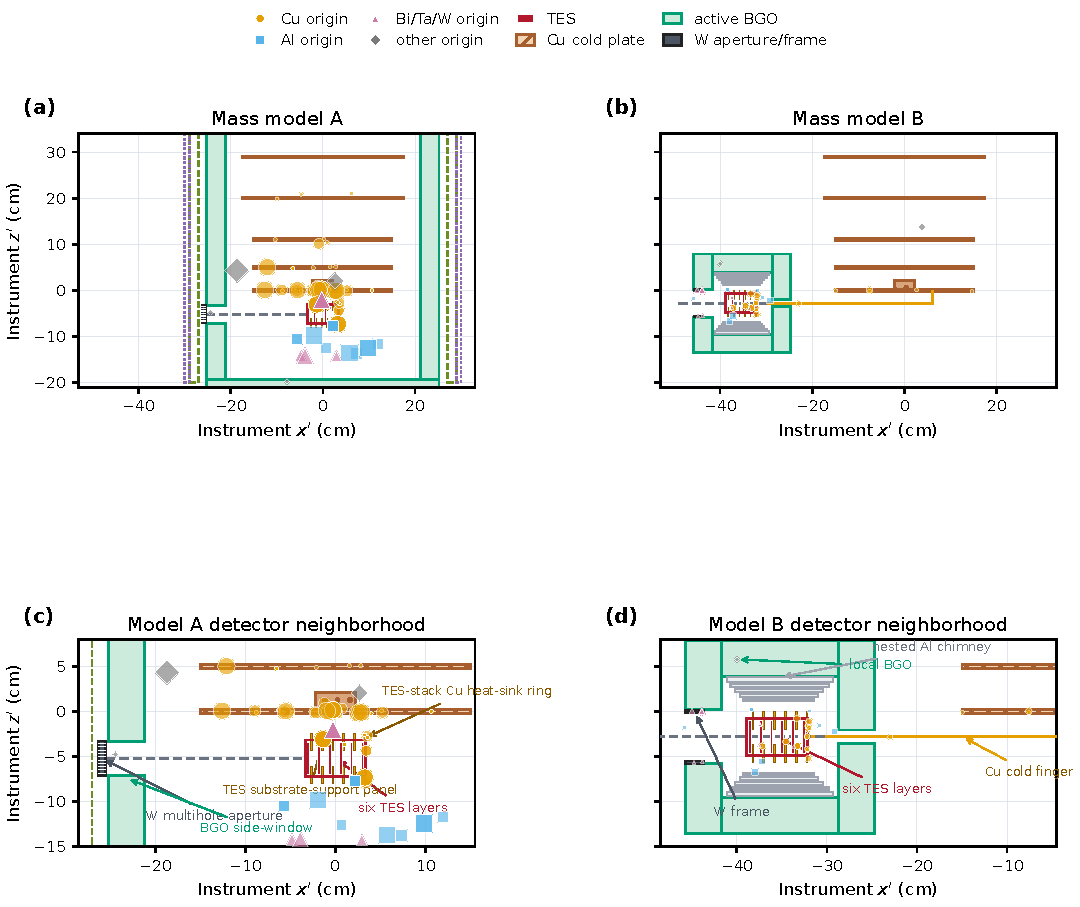
\includegraphics[width=\linewidth]{figures/section4_current/fig09_geometry_response_detailed.pdf}
\caption{Dimensionally aligned $x'$--$z'$ sections of the cold end and focal plane, overlaid with the parent-production positions of final delayed events. Panels (a) and (b) show mass models A and B over identical coordinate ranges and at the same scale; panels (c) and (d) show their detector neighbourhoods at a common physical scale. The drawings identify the staged copper cold plates, six-layer TES, active BGO, tungsten aperture/frame, model-B chimney and copper cold finger, and the model-A TES substrate-support copper panel, TES-stack copper heat-sink ring, and 50 mK MXC-stage copper cold plate. Each symbol marks the production position associated with a day-15 delayed event that survives the final selection; colour identifies the source material, and marker area follows the selected weighted rate on a common scale subject to a minimum display size. Sections are drawn to the transport-geometry dimensions; minor CSG apertures and service components are omitted for clarity.}
\label{fig:optimized_shield_background}
\end{figure}

\FloatBarrier

\subsection{Full-chain background and source redistribution in mass model B}
\label{subsec:optimized_fullchain}

Table~\ref{tab:optimized_cutflow} gives the mass-model-B day-15 direct,
no-coincidence cut flow.

Active BGO reduces the total background from 7,684 records and $2.384\cps$ to 137 records and $1.114\times10^{-2}\cps$, or 0.4672\% of the pre-veto rate. All 28,434 isolated focused-signal records in the measured window pass the active gate. The final Compton topology/aperture selection leaves 126 background records and retains 96.49\% of the active-veto weighted rate. It retains 27,936 focused records, corresponding to $15.085\pm0.045\,\mathrm{cm^2}$, 98.25\% of the measured-window signal area, and 99.75\% of model A's final effective area.

\begin{table}[H]
\centering
\caption{Mass model B response-convolved science-window cut flow. Background entries are day-15 direct, no-coincidence record counts and rates; signal entries give record counts and effective area.}
\label{tab:optimized_cutflow}
\footnotesize
\begin{tabular}{lccc}
\toprule
Stream & Pre-veto & After active BGO & Final topology/aperture \\
\midrule
Seven non-$\gamma$ prompt particle families & 1448 / $0.8787\cps$ & 3 / $1.811\times10^{-3}\cps$ & 3 / $1.811\times10^{-3}\cps$ \\
Atmospheric $\gamma$ & 2987 / $1.379\cps$ & 12 / $5.355\times10^{-3}\cps$ & 12 / $5.355\times10^{-3}\cps$ \\
Delayed activation & 3249 / $0.1256\cps$ & 122 / $3.971\times10^{-3}\cps$ & 111 / $3.581\times10^{-3}\cps$ \\
Total background & 7684 / $2.384\cps$ & 137 / $1.114\times10^{-2}\cps$ & 126 / $1.075\times10^{-2}\cps$ \\
Focused signal & 28434 / $15.35\,\mathrm{cm^2}$ & 28434 / $15.35\,\mathrm{cm^2}$ & 27936 / $15.085\,\mathrm{cm^2}$ \\
\bottomrule
\end{tabular}
\end{table}

The final model-B direct background contains $1.811\times10^{-3}\cps$ from
the seven non-$\gamma$ prompt particle families, $5.355\times10^{-3}\cps$ from atmospheric
$\gamma$ rays, and $3.581\times10^{-3}\cps$ from delayed
activation. Their shares are 16.85\%, 49.83\%, and 33.32\%, respectively.
Relative to mass model A, the delayed and atmospheric-$\gamma$ rates fall to
9.492\% and 34.92\%, and the total rate is $1.075\times10^{-2}\cps$, or
20.26\% of the model-A value, a factor of 4.94 lower. Table~\ref{tab:optimized_component_precision}
lists the component rates and finite-transport standard errors, and
Figure~\ref{fig:background_composition} compares the final fractional
compositions of the two models using the same categories.

\begin{table}[!ht]
\centering
\caption{Day-15 final direct-background composition and statistical uncertainty for mass model B. Standard errors and effective sample sizes are calculated from $\sum_i w_i^2$ for unequal event weights.}
\label{tab:optimized_component_precision}
\scriptsize
\resizebox{\linewidth}{!}{%
\begin{tabular}{lrrrrr}
\toprule
Component & Records & Rate / $\cps$ & Standard error / $\cps$ & $N_{\mathrm{eff}}$ & Total / \% \\
\midrule
Seven non-$\gamma$ prompt particle families & 3 & $1.811\times10^{-3}$ & $1.046\times10^{-3}$ & 3.00 & 16.85 \\
Atmospheric $\gamma$ & 12 & $5.355\times10^{-3}$ & $1.556\times10^{-3}$ & 11.84 & 49.83 \\
Delayed activation & 111 & $3.581\times10^{-3}$ & $5.370\times10^{-4}$ & 44.46 & 33.32 \\
\midrule
Total & 126 & $1.075\times10^{-2}$ & $1.950\times10^{-3}$ & 30.36 & 100.0 \\
\bottomrule
\end{tabular}}
\end{table}

Copper-derived events contribute $(2.27\pm0.43)\times10^{-3}\cps$, or
63.32\% of the final model-B delayed rate. The spatial-region contribution from
the DR/mixing chamber and staged cold plates falls from
$(1.21\pm0.27)\times10^{-2}\cps$ in mass model A to
$(1.4\pm1.1)\times10^{-4}\cps$ in mass model B. The
total delayed rate changes from $(3.77\pm0.46)\times10^{-2}$ to
$(3.58\pm0.54)\times10^{-3}\cps$.

Figure~\ref{fig:activation_origin_donuts_b} resolves the 111 final delayed-activation
origins in mass model B. The TES substrate-support Cu panels and TES Cu
heat-sink ring contribute 26.05\% and 25.73\%, respectively, or 51.78\%
together. The W focal-plane frame and the Al chimney shells, service lid, and annuli each
contribute 16.42\%. The TES bottom Cu cold-plate spoke, 50~mK mixing-chamber
Cu plate, and cold-link hardware contribute 5.72\%, 3.93\%, and 3.78\%,
respectively, while the TES-pixel Ta volumes and residual BGO side shield each
contribute about 1\%. The initiating primaries are dominated by protons
(57.89\%), followed by neutrons (20.81\%) and $\alpha$ particles (18.39\%);
$\gamma$ rays and leptons contribute 2.83\% and 0.09\%, respectively. Thus,
the residual delayed background in mass model B is concentrated in the TES
support panels and heat-sink ring, whereas the 50~mK mixing-chamber Cu plate
accounts for 3.93\%.

\begin{figure}[!htbp]
\centering
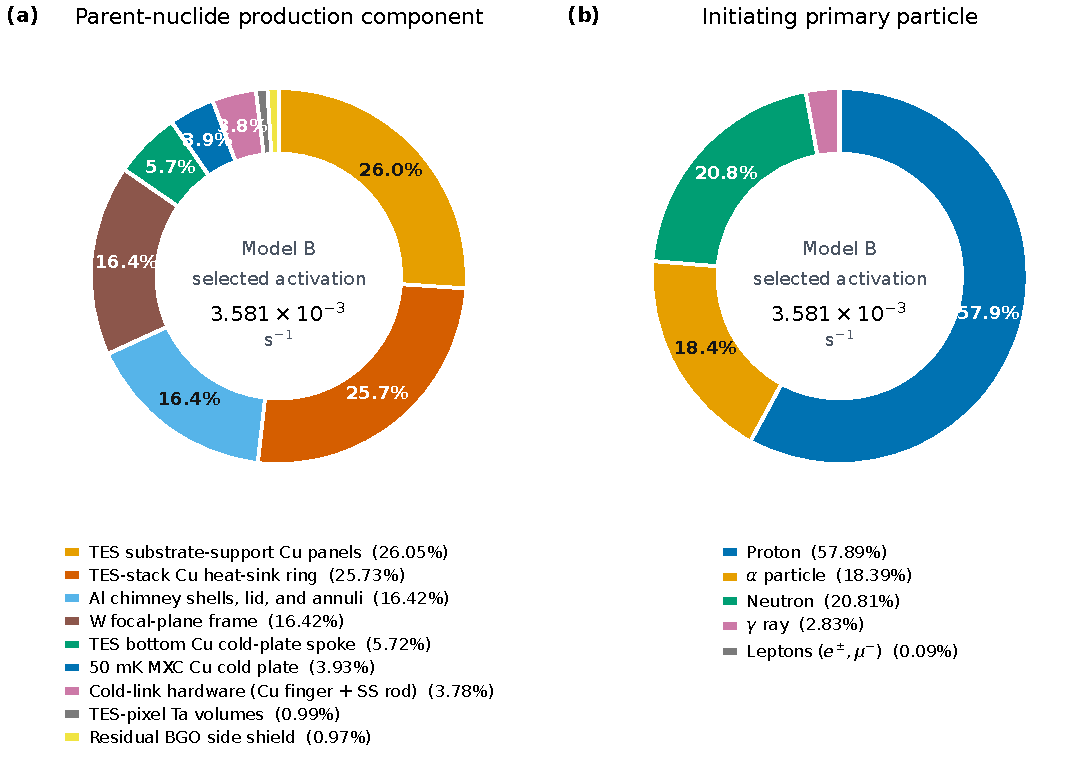
\includegraphics[width=0.96\linewidth]{figures/section4_current/fig_activation_origin_donuts_model_b.pdf}
\caption{Origins of the final day-15 delayed-activation background in mass model B. (a) Component in which the parent nuclide was produced. (b) Primary particle that initiated its production. Four Cu substrate-support panels (L2/L4/L5) are grouped, as are the Al chimney/port/lid/annulus volumes and the Cu-finger/SS-rod cold link; Ta pixels and BGO remain separate. Leptons combine $e^-$, $e^+$, and $\mu^-$. Each of the 111 records was reweighted by primary family to the current formal rate before aggregation. Both panels use $3.581\times10^{-3}\cps$ as their denominator.}
\label{fig:activation_origin_donuts_b}
\end{figure}

\begingroup

When grouped by parent nuclide, $^{62}$Cu is the largest single
delayed-background contributor in both mass models. Its weighted rate is
$1.774\times10^{-2}\cps$ in mass model A and
$1.238\times10^{-3}\cps$ in mass model B, accounting for 47.02\% and
34.58\% of the respective final delayed rates. Together, $^{61}$Cu,
$^{62}$Cu, and $^{64}$Cu contribute 65.50\% of the final delayed rate in mass
model A and 51.82\% in mass model B. Figure~\ref{fig:selected_delayed_parent_nuclides}
compares the leading parent-nuclide compositions.

\begin{figure}[!htbp]
\centering
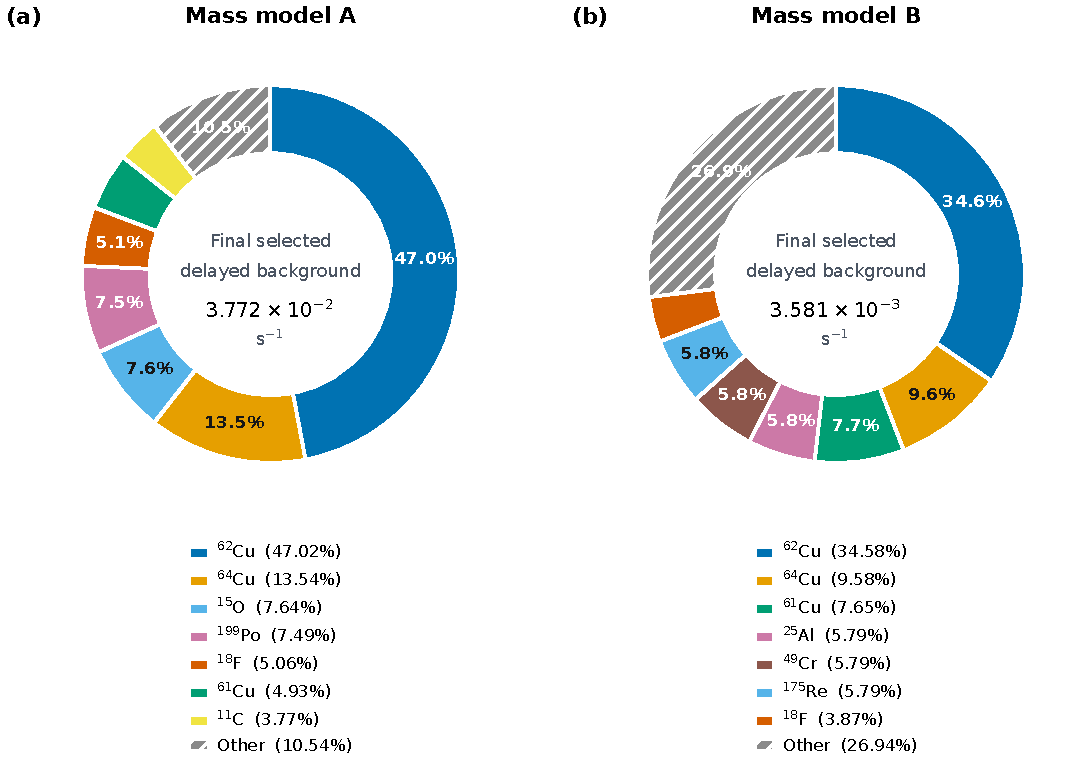
\includegraphics[width=0.96\linewidth]{figures/section4_current/fig_selected_delayed_parent_nuclide_donuts.pdf}
\caption{Parent-nuclide composition of the final selected day-15 delayed-activation background in (a) mass model A and (b) mass model B. All events have passed the TES response, the $510.58$--$511.42\keV$ science window, active anticoincidence, and the Compton topology/aperture selection. Sector area gives each parent nuclide's fraction of the corresponding final delayed rate. The seven leading parent nuclides are shown separately in each panel and the remainder is grouped as Other. Nuclides shared by the two panels use the same colours, and the total delayed-background rate is printed at each centre. The compact model-B origin records are reweighted to the current formal rate of each initiating particle family.}
\label{fig:selected_delayed_parent_nuclides}
\end{figure}
\endgroup

\FloatBarrier

\begin{figure}[H]
\centering
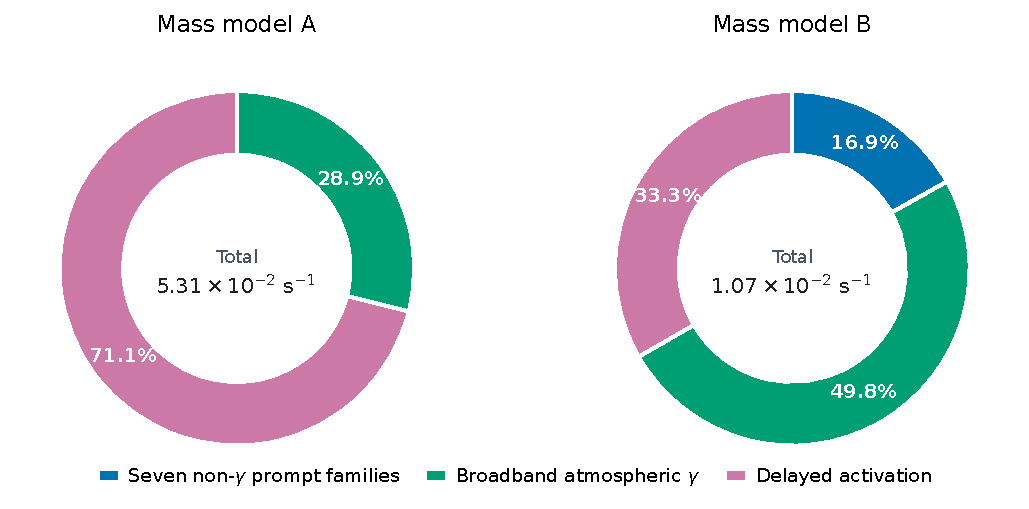
\includegraphics[width=0.92\linewidth]{figures/section4_current/fig09_background_composition.pdf}
\caption{Composition of the final direct background in the day-15 $510.58$--$511.42\keV$ science window after all selections. Sector area gives each physical component's fraction of the corresponding model total, shown at the centre; the same component colours are used in both panels.}
\label{fig:background_composition}
\end{figure}

Figure~\ref{fig:day15_selection_spectra} shows the day-15 spectra before active
anticoincidence, after the active gate, and after the final Compton selection.
The 480--550 keV band provides a selection diagnostic independent of the
narrow-window integral. In mass model A, its weighted rate changes from
$10.80\cps$ to $0.1408\cps$ and then $0.1213\cps$; the corresponding
model-B rates are $4.922$, $0.07353$, and $0.06552\cps$. The same ordering
appears in the science-window cut flows: active anticoincidence supplies the
dominant suppression, and the Compton topology/aperture selection makes a
smaller correction to the residual.

\begin{figure}[!ht]
\centering
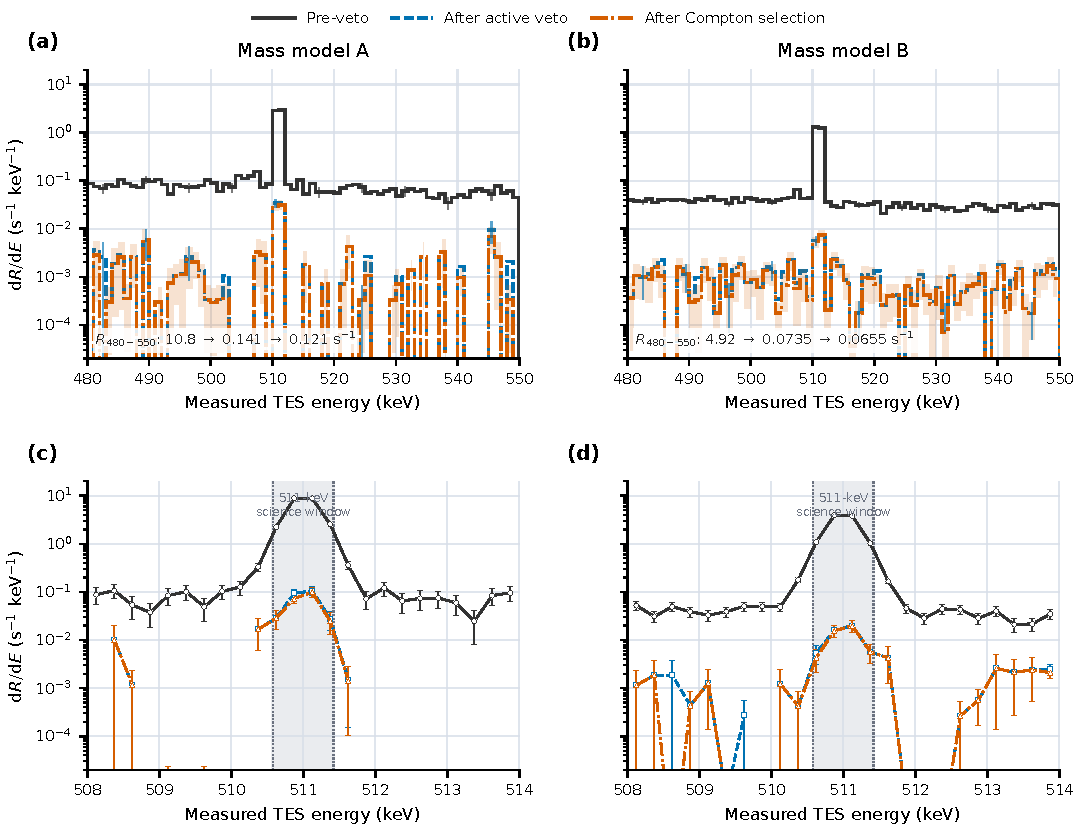
\includegraphics[width=\linewidth]{figures/section4_current/fig05_day15_selection_spectra_current.pdf}
\caption{Day-15 detector-side differential count-rate spectra through the event-selection chain. Panels (a) and (b) show 480--550 keV for mass models A and B; four adjacent 0.25 keV analysis bins are summed into each 1 keV display bin. Panels (c) and (d) show 508--514 keV at the native 0.25 keV binning; the shaded interval and dotted boundaries mark the $[510.58,511.42)\keV$ science window. Curves show the direct, no-coincidence background before active anticoincidence, after active anticoincidence, and after the final Compton topology/aperture selection. The translucent band in the 480--550 keV panels and the bin-wise error bars in the zoom panels show finite-transport $1\sigma$ uncertainties from $\sqrt{\sum_i w_i^2}$. Zero-weight bins are left blank, without smoothing or pseudocounts. The ordinate is the detector differential count rate after transport and TES-response convolution.}
\label{fig:day15_selection_spectra}
\end{figure}

The larger reduction in delayed activation shifts the dominant component from
delayed activation in model A to atmospheric $\gamma$ rays in model B.

\FloatBarrier

\subsection{Common-time fold and cumulative counts}
\label{subsec:mission_fold_validation}

At the day-0, 5, 10, 15, and 20 anchors, Poisson arrivals are regenerated from the physical component rates and passed through the common time grouping, detector response, active anticoincidence, and Compton selection. The ratio of the common-time final rate to the direct rate defines $\widehat\rho_g$, and focused-signal replay gives the accidental survival $\widehat\eta_g$; both are interpolated to the 81 mission nodes. The model-A $\widehat\rho_g$ values span 0.9307--1.006, and the model-B values span 0.9901--1.029 (Figure~\ref{fig:common_time_anchors}).

All five replay rates agree with the analytic curve within $2\sigma$ using
replay-only errors, confirming common-time closure.

The focused-signal $\widehat\eta_g$ values span 0.9681--0.9704 for mass model A and 0.9955--0.9958 for mass model B; their day-15 values are 0.9682 and 0.9955. The higher model-B survival follows from lower coincidence occupancy rather than a different signal selection. The interpolated $\rho_g$ and $\eta_g$ values are combined with the same trajectory transmission and component responses and integrated over 81 nodes at 0.25 d spacing.

Combining the day-15 conditional survival fractions with the isolated-event final effective areas and the atmospheric transmission at that node gives final signal rates of $1.805\times10^{-3}$ and $1.851\times10^{-3}\cps$ for mass models A and B, respectively, at the reference flux defined in Section~\ref{sec:requirements}. Mass model B has a slightly smaller isolated-event effective area but a smaller accidental-coincidence loss, and therefore a slightly higher final reference signal rate.

At 20 d, the expected signal/background counts are 3098/$87{,}632$ for mass
model A and 3176/$18{,}569$ for mass model B. Atmospheric $\gamma$ rays and the
remaining background contribute $25{,}760$/$61{,}872$ counts in model A and
$9{,}359$/$9{,}209$ in model B. The model-B cumulative background is 21.19\%
of the model-A value.

\subsection{Mission significance and minimum resolvable line flux}
\label{subsec:final_mission_performance}

Figure~\ref{fig:optimized_mission_significance} and
Table~\ref{tab:primary_sensitivity} summarize the mission performance. At
$\fref$, the 20 d counting significances are 10.47 for mass model A and
23.31 for mass model B. The corresponding $3\sigma$ minimum resolvable
top-of-atmosphere fluxes are $(6.88\pm0.51)\times10^{-5}$ and
$(3.09\pm0.28)\times10^{-5}\phcms$.

\begin{figure}[!ht]
\centering
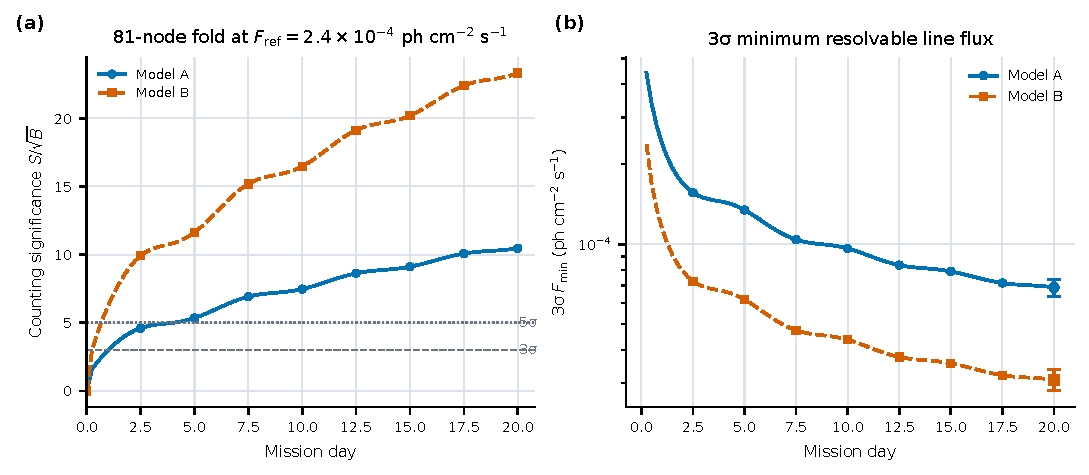
\includegraphics[width=0.98\linewidth]{figures/section4_reference_flux_20260830/fig10_mission_performance_gaussian.pdf}
\caption{Conditional 81-node mission performance of mass models A and B. (a)
Counting significance at the top-of-atmosphere reference flux
$\fref=2.4\times10^{-4}\phcms$; horizontal lines mark $3\sigma$ and
$5\sigma$. (b) Corresponding $3\sigma$ minimum resolvable top-of-atmosphere
flux. Both designs use the same source, detector response, science window,
timing, topology/aperture test, and atmospheric-transmission conventions; their
entrances, local tungsten structures, and geometry-specific active channels
differ.}
\label{fig:optimized_mission_significance}
\end{figure}

\begin{table}[!ht]
\centering
\caption{Conditional 20 d on-source projection for mass models A and B.}
\label{tab:primary_sensitivity}
\footnotesize
\resizebox{\linewidth}{!}{%
\begin{tabular}{lrr}
\toprule
Quantity & Mass model A & Mass model B \\
\midrule
Selected effective area / $\mathrm{cm^2}$ & $15.123\pm0.045$ & $15.085\pm0.045$ \\
Day-15 direct background / $\cps$ & $5.306\times10^{-2}$ & $1.075\times10^{-2}$ \\
Day-15 signal at $\fref$ / $\cps$ & $1.805\times10^{-3}$ & $1.851\times10^{-3}$ \\
20 d background counts & 87632 & 18569 \\
20 d signal counts at $\fref$ & 3098 & 3176 \\
$Z_{20\mathrm d}=N_s/\sqrt{N_b}$ & 10.47 & 23.31 \\
$T_{3\sigma}$ at $\fref$ / d & 0.997 & 0.248 \\
$T_{5\sigma}$ at $\fref$ / d & 4.00 & 0.673 \\
$F_{3\sigma}(20\,\mathrm d)$ / $\phcms$ &
$(6.88\pm0.51)\times10^{-5}$ &
$(3.09\pm0.28)\times10^{-5}$ \\
$F_{5\sigma}(20\,\mathrm d)$ / $\phcms$ &
$(1.147\pm0.085)\times10^{-4}$ &
$(5.15\pm0.47)\times10^{-5}$ \\
\bottomrule
\end{tabular}}
\end{table}

\FloatBarrier

The flux-threshold ratio separates into cumulative-background and cumulative-signal-kernel terms. The 20 d model-B background is 21.19\% of the model-A value, while its cumulative signal kernel is 1.025 times the model-A value:
\begin{equation}
 \frac{F_{\min,A}}{F_{\min,B}}
 =\sqrt{\frac{N_{b,A}}{N_{b,B}}}\frac{K_B^{20\mathrm d}}{K_A^{20\mathrm d}}
 \simeq2.172\times1.025
 \simeq2.227 .
 \label{eq:fmin_ratio_decomposition}
\end{equation}
Here $K_g^{20\mathrm d}$ is the cumulative signal kernel integrated over the 81 nodes. Equation~\eqref{eq:fmin_ratio_decomposition} shows that most of the 2.227-fold threshold difference follows from the square root of the background ratio, with a smaller correction from the cumulative signal kernel.

Mass model B retains 99.75\% of the focused effective area of mass model A and reduces the 20 d cumulative background and $3\sigma$ flux threshold to 21.19\% and 44.90\%, respectively.

\FloatBarrier

\section{Response screening in orbital and lunar environments}
\label{sec:environment_screening}

The balloon calculation establishes the model-B response and trajectory-folded
sensitivity. To identify which radiation fields would limit the same
detector response in other mission environments, we traced the selected events
back to their primary particle types and energies and reweighted them with
source spectra for LEO, the lunar surface, and Sun--Earth L2. The calculation
therefore shows how a change in radiation environment acts on the established
TES response and helps set priorities for detailed follow-up simulations.

\subsection{Spectral reweighting}

We considered four representative source fields: quiet, near-equatorial LEO at
530\,km outside the SAA; an exposed lunar surface; and two Sun--Earth L2
conditions representing solar maximum and solar minimum. The LEO spectra use
the components adopted in low-Earth-orbit gamma-ray background studies
\cite{Cumani2019LEO}. The lunar field combines the upward REDMoon spectrum for
Apollo-17 regolith with the cosmic gamma-ray sky visible from the surface
\cite{Dobynde2021REDMoon}. The L2 fields contain gamma rays, protons, alpha
particles, electrons, and positrons, with GCR spectra appropriate to the two
solar-modulation conditions
\cite{Lotti2021Athena,Usoskin2005,Kuznetsov2017}.

For the prompt-gamma background, each selected event retains the energy of
its primary photon. A selected delayed event is linked instead to the
activation-production energy distribution for the same incident particle,
parent nuclide, and production region. At those primary energies, each balloon
event weight is multiplied by the ratio of the target spectrum to the balloon
spectrum. The two components are then normalized to the formal day-15 rates of
mass model B: $5.355\times10^{-3}\cps$ for prompt gamma rays and
$3.581\times10^{-3}\cps$ for delayed activation. The principal response
bands shown in Figure~\ref{fig:environment_transfer} are
$0.598$--$29.6$\,MeV for selected prompt gamma rays and
$1.37$--$48.4$\,GeV for proton-induced delayed background.

The seven non-gamma prompt families contribute 16.85\% of the balloon
background. Because the transfer response lacks an independent prompt-positron
energy kernel, their aggregate rate follows the combined prompt-gamma and
delayed-activation scaling; no family-resolved target-environment rates are
reported.

All scenarios use the same 20\,d exposure and the effective area of mass model
B. The screening flux is anchored to the balloon result of
$3.089\times10^{-5}\phcms$, scaled with the square root of the reweighted
background and corrected for the cumulative signal loss of the balloon
trajectory relative to an unattenuated, continuously on-source observation.
The balloon value is quoted at the top of the atmosphere, whereas the other
values refer to the local instrument incident plane.

\begin{figure}[!ht]
\centering
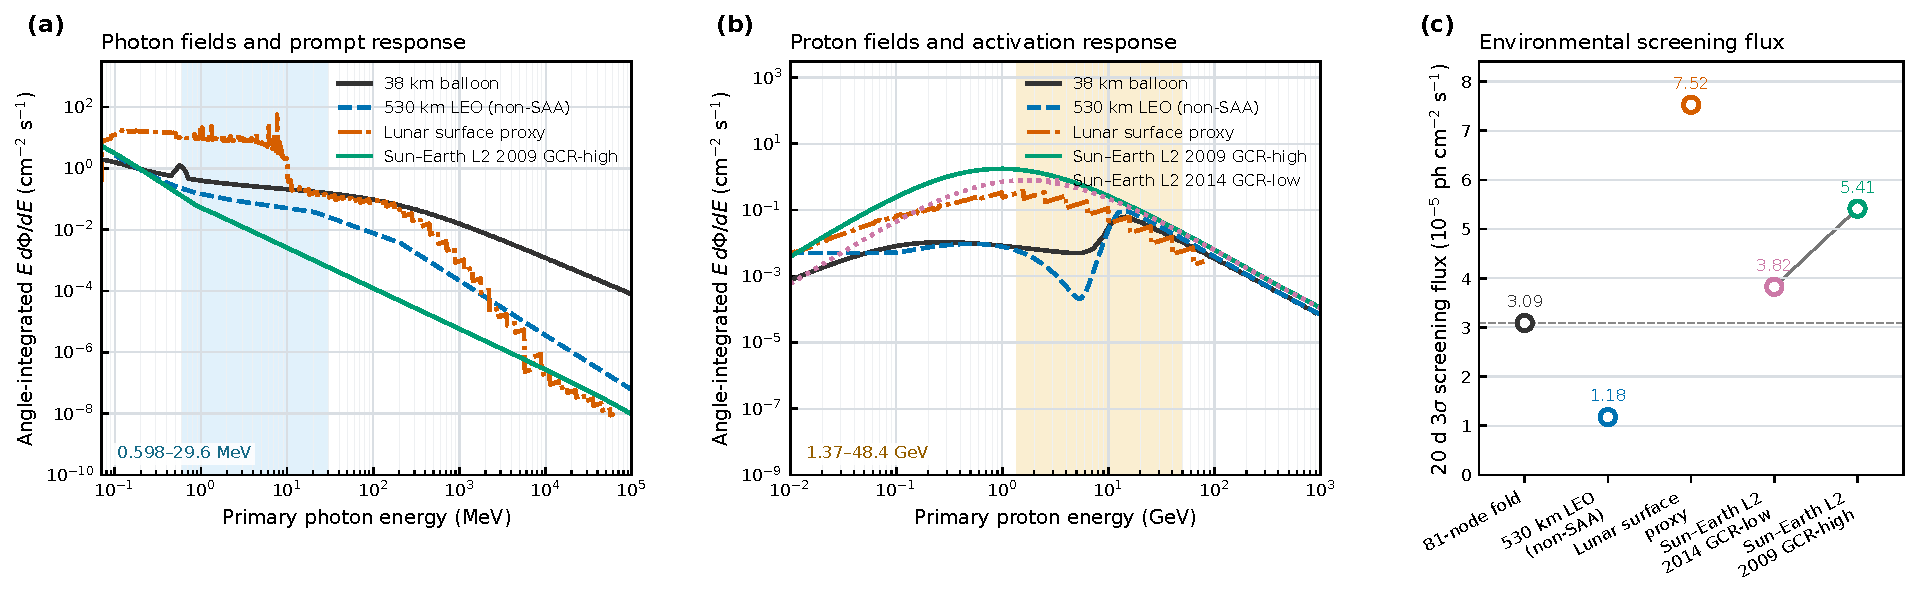
\includegraphics[width=\linewidth]{figures/environment_screening_20260830/fig11_environment_transfer_en.pdf}
\caption{Environmental spectral reweighting for mass model B. (a) Gamma-ray
source spectra; the shaded band is the principal primary-energy range of the
selected prompt-gamma events ($0.598$--$29.6$\,MeV). (b) Proton spectra; the
shaded band is the principal response range of the proton-induced delayed
background ($1.37$--$48.4$\,GeV). (c) The 20\,d, $3\sigma$ screening flux
anchored to the balloon result. The balloon value is defined at the top of the
atmosphere and the others at the local instrument incident plane.}
\label{fig:environment_transfer}
\end{figure}

\subsection{Screening results for LEO, the lunar surface, and L2}

\begin{table}[!ht]
\centering
\caption{Spectral-reweighting screen for mass model B in different radiation
environments. The third column gives the combined prompt-gamma and
delayed-activation rate relative to the balloon reference; the last column is
the $3\sigma$ screening flux for the same 20\,d exposure.}
\label{tab:environment_screening}
\small
\resizebox{\linewidth}{!}{%
\begin{tabular}{llrr}
\toprule
Scenario & Source-field proxy & Reweighted background/balloon & 20\,d $3\sigma$ screening flux / $\phcms$ \\
\midrule
Balloon reference & formal 81-node trajectory & 1.000 & $3.089\times10^{-5}$ \\
530 km LEO & near-equatorial, quiet non-SAA & 0.5627 & $1.176\times10^{-5}$ \\
Exposed lunar surface & REDMoon Apollo-17 regolith & 23.02 & $7.525\times10^{-5}$ \\
Sun--Earth L2 (2014) & solar maximum, GCR-low & 5.946 & $3.824\times10^{-5}$ \\
Sun--Earth L2 (2009) & solar minimum, GCR-high & 11.92 & $5.414\times10^{-5}$ \\
\bottomrule
\end{tabular}}
\end{table}

For quiet non-SAA LEO, the reweighted background is 0.5627 times the balloon
reference. After removing the signal loss associated with the balloon
atmosphere and observing trajectory, the 20\,d screening flux is
$1.176\times10^{-5}\phcms$. Thus, in quiet orbital segments, the current source
field produces less background in mass model B than the balloon environment.
For a 550\,km equatorial orbit, Cumani et al. estimated that the region occupied
by trapped particles above 0.1\,MeV accounts for about 18\% of the orbital
period; science observations are normally suspended during these SAA passages
\cite{Cumani2019LEO}. A 20\,d calendar interval would therefore provide about
16.4\,d of live exposure before any post-SAA cooldown. The 20\,d value in
Table~\ref{tab:environment_screening} denotes live science exposure. The next
LEO calculation should concentrate on activation by SAA and trapped particles
and on the delayed background after an SAA passage.

For the exposed lunar surface, the reweighted background rises to 23.02 times
the balloon reference and the screening flux becomes
$7.525\times10^{-5}\phcms$. The increase is driven mainly by upward regolith
radiation in the response band of the selected gamma-ray events. A lunar
application therefore requires a local gamma-ray field that couples the
regolith, detector, and lander structure rather than an isolated-payload model.

At Sun--Earth L2, the result follows solar modulation. The 2014
solar-maximum/GCR-low field gives $3.824\times10^{-5}\phcms$, whereas the 2009
solar-minimum/GCR-high field gives $5.414\times10^{-5}\phcms$. Their ordering
tracks the proton spectra and identifies GCR-proton activation as the main L2
driver. Because the present delayed response is supported by a limited set of
activation templates, these values are most useful for setting the priority of
a dedicated proton-activation calculation.

The reweighting therefore points to a different next step in each environment:
an orbital history including SAA and trapped particles for LEO, local
regolith--lander coupling for the lunar surface, and higher-statistics GCR
proton activation at L2. Matched prompt, activation, and delayed transport in
each target environment is the next step toward mission-level performance
predictions.

\FloatBarrier

\section{Summary}
\label{sec:summary}

The day-15 selected background rate of mass model A is
$5.306\times10^{-2}\cps$, with delayed activation as the largest component.
Independent spatial and material projections assign 32.18\% of the delayed
rate to the DR mixing chamber and staged cold region and 70.87\% to copper,
respectively. The leading structures are the
50 mK copper cold plate, the TES substrate-support copper panels, and the TES
copper heat-sink ring. The science-window background is governed by the
distance, direct lines of sight, and shield coverage between activated material
and the TES.

Mass model B places the six TES layers laterally in a BGO-surrounded chimney.
Its final day-15 background rate is $1.075\times10^{-2}\cps$, composed of
49.83\% atmospheric gamma rays, 33.32\% delayed activation, and
16.85\% from the seven non-gamma prompt families. The active BGO reduces the
direct science-window rate from $2.384$ to
$1.114\times10^{-2}\cps$, after which the topology and aperture selection
leaves $1.075\times10^{-2}\cps$. The selected effective area of mass model B
is 99.75\% of that of mass model A, while its final topology and aperture
selection retains 98.25\% of the focused signal in its own measured-energy
window. Its 20\,d, top-of-atmosphere $3\sigma$ minimum resolvable line flux is
$(3.09\pm0.28)\times10^{-5}\phcms$, a factor of 2.23 lower than for mass
model A.

The results support two priorities: reduce coupling between the TES and
activation-prone near-field structures by reducing or relocating them and
blocking direct lines of sight, and maximize active-BGO coverage within the
optical path. In mass model B, the TES
substrate-support copper panels and copper heat-sink ring still account for
51.78\% of the residual delayed background and are the direct targets of the
next near-field redesign.

\section{Outlook}
\label{sec:outlook}

The most immediate extension is a dedicated LEO satellite. The preliminary
screening in Section~\ref{sec:environment_screening} identifies quiet non-SAA
orbital segments as a priority for a complete mission design. Compared with a
finite-duration balloon flight, a LEO satellite avoids attenuation through the
balloon atmospheric column and can extend live exposure from months to years.
The orbit, shielding geometry, and observing schedule should be designed
together: a near-equatorial, low-inclination orbit, shutdown during SAA
passages, planned post-SAA cooldown, reduced activation near the TES, and wider
BGO solid-angle coverage are the first parameters to study. A mission model
including the spacecraft, Earth-albedo radiation, trapped-particle and SAA
histories, Earth occultation, and source visibility can then determine how far
long-duration operation lowers the minimum resolvable line flux.

A lunar instrument is a more exploratory, longer-term option. The simple
spectral reweighting in Section~\ref{sec:environment_screening} exposes the
pressure from upward regolith gamma rays, but it does not use the additional
mass and installation volume that a lunar platform may provide. If those
resources are available, the TES, cryogenic system, and lander can be optimized
in a coupled mass model. Directional lower-hemisphere shielding, active
anticoincidence below and beside the focal plane, and shadowing by the lander
could reduce direct coupling of the upward regolith field to the TES. Coupled
regolith--lander--instrument transport will be needed to determine whether such
a design can suppress the regolith-albedo background while benefiting from
unattenuated celestial photons and long cumulative exposure.

\newpage
\begin{samepage}
A further detector-level study should address neutron elastic scattering in
the cryogenic Si wafer and nearby focal-plane supports. Nuclear-recoil energy
deposited in these volumes can generate athermal and thermal phonons; if a
fraction couples to the TES, the response may appear as a non-photon pulse or
as thermal cross-talk \cite{Agnese2018NuclearRecoil,Hull2023ThermalBackground}.
Coupled neutron-transport, substrate-phonon, TES thermal-network, and measured
pulse-template studies, together with neutron-beam calibration, are needed to
determine whether such events can be reconstructed in the 511 keV science
window and whether their pulse shapes permit rejection.
\end{samepage}

\section*{Declarations}
\textbf{Ethics approval and consent to participate} Not applicable.

\begin{thebibliography}{99}

\bibitem{Prantzos2011}
N. Prantzos, C. Boehm, A.M. Bykov, R. Diehl, K. Ferriere, N. Guessoum, P. Jean, J. Knoedlseder, A. Marcowith, I.V. Moskalenko, A. Strong, G. Weidenspointner, The 511 keV emission from positron annihilation in the Galaxy, Rev. Mod. Phys. 83 (2011) 1001--1056, doi:10.1103/RevModPhys.83.1001.

\bibitem{Jean2006}
P. Jean, J. Knoedlseder, V. Lonjou, M. Allain, J.-P. Roques, G.K. Skinner, B.J. Teegarden, G. Vedrenne, P. von Ballmoos, B. Cordier, P. Caraveo, R. Diehl, P. Durouchoux, P. Leleux, R. Schanne, G. Weidenspointner, Spectral analysis of the Galactic $e^+e^-$ annihilation emission, Astron. Astrophys. 445 (2006) 579--589, doi:10.1051/0004-6361:20053765.

\bibitem{Kierans2020}
C.A. Kierans, S.E. Boggs, A. Zoglauer, A.W. Lowell, C. Sleator, J. Beechert, T.J. Brandt, P. Jean, H. Lazar, J. Roberts, T. Siegert, J.A. Tomsick, P. von Ballmoos, Detection of the 511 keV Galactic positron annihilation line with COSI, Astrophys. J. 895 (2020) 44, doi:10.3847/1538-4357/ab89a9.

\bibitem{Siegert2016AA}
T. Siegert, R. Diehl, G. Khachatryan, M.G.H. Krause, F. Guglielmetti, J. Greiner, A.W. Strong, X. Zhang, Gamma-ray spectroscopy of positron annihilation in the Milky Way, Astron. Astrophys. 586 (2016) A84, doi:10.1051/0004-6361/201527510.

\bibitem{Siegert2016V404}
T. Siegert, R. Diehl, J. Greiner, M.G.H. Krause, A.M. Beloborodov, M. Cadolle Bel, F. Guglielmetti, J. Rodriguez, A.W. Strong, X. Zhang, Positron annihilation signatures associated with the outburst of the microquasar V404 Cygni, Nature 531 (2016) 341--343, doi:10.1038/nature16978.

\bibitem{Knodlseder2005AllSky}
J. Knoedlseder, P. Jean, V. Lonjou, G. Weidenspointner, N. Guessoum, R. Diehl, W. Gillard, M.J. Harris, G.K. Skinner, P. von Ballmoos, G. Vedrenne, P. Caraveo, B. Cordier, V. Schoenfelder, B.J. Teegarden, The all-sky distribution of 511 keV electron-positron annihilation emission, Astron. Astrophys. 441 (2005) 513--532, doi:10.1051/0004-6361:20042063.

\bibitem{Yoneda2025}
H. Yoneda, T. Siegert, S. Mittal, Imaging the positron annihilation line with 20 years of INTEGRAL/SPI observations, arXiv:2509.01066, 2025.

\bibitem{Siegert2020COSI}
T. Siegert, S.E. Boggs, J.A. Tomsick, A.C. Zoglauer, C.A. Kierans, C.C. Sleator, J. Beechert, T.J. Brandt, P. Jean, H. Lazar, A.W. Lowell, J.M. Roberts, P. von Ballmoos, Imaging the 511 keV positron annihilation sky with COSI, Astrophys. J. 897 (2020) 45, doi:10.3847/1538-4357/ab9607.

\bibitem{Siegert2019Kinematics}
T. Siegert, R. Diehl, G. Khachatryan, M.G.H. Krause, F. Guglielmetti, J. Greiner, A.W. Strong, X. Zhang, Constraints on positron annihilation kinematics in the inner Galaxy, Astron. Astrophys. 627 (2019) A126, doi:10.1051/0004-6361/201833856.

\bibitem{DeCesare2011}
G. De Cesare, Searching for the 511 keV annihilation line from galactic compact objects with the IBIS gamma ray telescope, Astron. Astrophys. 531 (2011) A56, doi:10.1051/0004-6361/201116516.

\bibitem{Barriere2009Laue}
N.M. Barriere, L. Natalucci, N. Abrosimov, P. von Ballmoos, P. Bastie, P. Courtois, M. Jentschel, J. Knodlseder, J. Rousselle, P. Ubertini, Soft gamma-ray optics: new Laue lens design and performance estimates, arXiv:0910.0488, 2009.

\bibitem{Barriere2011LauePrototype}
N.M. Barriere, J.A. Tomsick, S.E. Boggs, A. Lowell, P. von Ballmoos, Developing a second generation Laue lens prototype: high reflectivity crystals and accurate assembly, arXiv:1111.6700, 2011.

\bibitem{Weidenspointner2006MAX}
G. Weidenspointner, C.B. Wunderer, N. Barriere, A. Zoglauer, P. von Ballmoos, Monte Carlo study of detector concepts for the MAX Laue Lens gamma-ray telescope, arXiv:astro-ph/0603152, 2006.

\bibitem{Shirazi2023}
F. Shirazi, E. Gau, M.A. Hossen, D. Becker, D. Schmidt, D. Swetz, D. Bennett, D. Braun, F. Kislat, J. Gard, J. Mates, J. Weber, N.R. Cavero, S. Chun, L. Lisalda, A. West, B. Dev, F. Ferrer, R. Bose, J. Ullom, H. Krawczynski, The 511-CAM Mission: A pointed 511 keV gamma-ray telescope with a focal plane detector made of stacked transition edge sensor microcalorimeter arrays, J. Astron. Telesc. Instrum. Syst. 9 (2023) 024006, doi:10.1117/1.JATIS.9.2.024006.

\bibitem{Zhang2022TESGamma}
S. Zhang, J.-K. Xia, T. Sun, et al., Transition edge sensor based detector: from X-ray to gamma-ray, arXiv:2204.00010, 2022.

\bibitem{Hu2026}
K. Hu, M. Fritts, D. Becker, D. Schmidt, F. Zhou, A. Dasgupta, F. Kislat, M. Keller, S. Chun, A.G. Detoito, E. Gau, X. Jin, D. Bennett, D. Braun, J. Gard, J.A.B. Mates, J. Nobles, D. Radomski, N. Rodriguez Cavero, R. Snodgrass, D. Swetz, J. Ullom, S. Vengalil Menon, J. Weber, K. Wimalasena, H. Krawczynski, Design of a mission to measure the shape and substructure of the 511 keV gamma-ray line from the center of the Milky Way, J. Astron. Telesc. Instrum. Syst. 12 (2026) 025002, doi:10.1117/1.JATIS.12.2.025002.

\bibitem{Gallego2025Balloon}
S. Gallego, U. Oberlack, J. Lommler, C.M. Karwin, A. Zoglauer, P. Jean, P. von Ballmoos, C. Kierans, C.C. Sleator, J.A. Tomsick, S.E. Boggs, Bottom-up background simulations of the 2016 COSI balloon flight, Astrophys. J. 986 (2025) 116, doi:10.3847/1538-4357/add6a0.

\bibitem{Tian2026DIXE}
R. Tian, J. Mao, J. Liu, H. Jin, W. Cui, Simulation of non-X-ray background for the DIffuse X-ray Explorer (DIXE) mission, arXiv:2604.13569, 2026.

\bibitem{Caputo2017}
R. Caputo, F. Kislat, J. Racusin, on behalf of the AMEGO Team, AMEGO: Simulations of the instrument performance, Proc. 35th International Cosmic Ray Conference, PoS(ICRC2017) 783 (2018), doi:10.22323/1.301.0783.

\bibitem{Gottardi2021TESReview}
L. Gottardi, K. Nagayoshi, A review of X-ray microcalorimeters based on superconducting transition edge sensors for astrophysics and particle physics, Applied Sciences 11 (2021) 3793, doi:10.3390/app11093793.

\bibitem{Yan2019TaHeatCapacity}
D. Yan, L.M. Gades, T. Guruswamy, U.M. Patel, O. Quaranta, A. Miceli, Modelling a transition-edge sensor X-ray microcalorimeter linear array for Compton profile measurements and energy dispersive diffraction, IEEE Trans. Appl. Supercond. 29(5) (2019) 1--4, doi:10.1109/TASC.2019.2906255.

\bibitem{Xie2026AlMn}
L. Xie, Y. Zhang, Z. Li, Z. Liu, S. Shu, J. Zhou, X. Li, H. Li, H. Gao, Y. Gu, X. Lu, Y. Zhao, C. Liu, Beyond one-thousandth energy resolution with an AlMn TES detector, arXiv:2602.11728, 2026.

\bibitem{Vavagiakis2017AlMnMagnetic}
E.M. Vavagiakis, S.W. Henderson, K. Zheng, H.-M. Cho, N.F. Cothard, B. Dober, S.M. Duff, P.A. Gallardo, G. Hilton, J. Hubmayr, K.D. Irwin, B.J. Koopman, D. Li, F. Nati, M.D. Niemack, C.D. Reintsema, S. Simon, J.R. Stevens, A. Suzuki, B. Westbrook, Magnetic sensitivity of AlMn TESes and shielding considerations for next-generation CMB surveys, arXiv:1710.08456, 2017.

\bibitem{NISTXCOM}
J.H. Hubbell, S.M. Seltzer, XCOM: Photon Cross Section Database, NIST Standard Reference Database 8 (XGAM), National Institute of Standards and Technology, doi:10.18434/T48G6X.

\bibitem{Agostinelli2003}
S. Agostinelli, J. Allison, K. Amako, et al., Geant4---a simulation toolkit, Nucl. Instrum. Methods Phys. Res. A 506 (2003) 250--303, doi:10.1016/S0168-9002(03)01368-8.

\bibitem{Allison2016}
J. Allison, K. Amako, J. Apostolakis, et al., Recent developments in Geant4, Nucl. Instrum. Methods Phys. Res. A 835 (2016) 186--225, doi:10.1016/j.nima.2016.06.125.

\bibitem{SanchezDelRio2011XOP}
M. Sanchez del Rio, R.J. Dejus, XOP v2.4: recent developments of the x-ray optics software toolkit, Proc. SPIE 8141 (2011) 814115, doi:10.1117/12.893911.

\bibitem{Guan2023BraggReflection}
F. Guan, M. Asai, D.A. Bartkoski, M. Kleckner, Z. Harel, M. Salehpour, Adding the X-ray Bragg reflection physical process in crystal to the Geant4 Monte Carlo simulation toolkit, part I: reflection from a crystal slab, Precision Radiation Oncology 7(1) (2023) 59--66.

\bibitem{Reiazi2025G4BraggReflection}
R. Reiazi, D. Lee, D. Bartkoski, M. Kleckner, M. Salehpour, G4BraggReflection for accurate modeling of Bragg reflection in perfect and mosaic crystals, J. Phys. D: Appl. Phys. 58 (2025) 295102, doi:10.1088/1361-6463/aded1d.

\bibitem{Zoglauer2006}
A. Zoglauer, R. Andritschke, F. Schopper, MEGAlib: The Medium Energy Gamma-ray Astronomy Library, New Astron. Rev. 50 (2006) 629--632, doi:10.1016/j.newar.2006.06.049.

\bibitem{Sato2015EXPACS}
T. Sato, Analytical model for estimating terrestrial cosmic ray fluxes nearly anytime and anywhere in the world: extension of PARMA/EXPACS, PLoS ONE 10 (2015) e0144679, doi:10.1371/journal.pone.0144679.

\bibitem{Sato2016PARMA4}
T. Sato, Analytical model for estimating the zenith angle dependence of terrestrial cosmic ray fluxes, PLoS ONE 11 (2016) e0160390, doi:10.1371/journal.pone.0160390.

\bibitem{Kondev2021NUBASE}
F.G. Kondev, M. Wang, W.J. Huang, S. Naimi, G. Audi, The NUBASE2020 evaluation of nuclear physics properties, Chinese Phys. C 45 (2021) 030001, doi:10.1088/1674-1137/abddae.

\bibitem{Kierans2017}
C.A. Kierans, S.E. Boggs, J.-L. Chiu, A. Lowell, C. Sleator, J.A. Tomsick, A. Zoglauer, M. Amman, H.-K. Chang, C.-H. Tseng, C.-Y. Yang, C.-H. Lin, P. Jean, P. von Ballmoos, The 2016 Super Pressure Balloon flight of the Compton Spectrometer and Imager, arXiv:1701.05558, 2017.

\bibitem{Cumani2019LEO}
P. Cumani, M. Hernanz, J. Kiener, V. Tatischeff, A. Zoglauer,
Background for a gamma-ray satellite on a low-Earth orbit,
Exp. Astron. 47 (2019) 273--302,
doi:10.1007/s10686-019-09624-0.

\bibitem{Dobynde2021REDMoon}
M.I. Dobynde, J. Guo,
Radiation environment at the surface and subsurface of the Moon:
model development and validation,
J. Geophys. Res. Planets 126 (2021) e2021JE006930,
doi:10.1029/2021JE006930.

\bibitem{Takahashi2007HXD}
T. Takahashi et al., Hard X-Ray Detector (HXD) on Board Suzaku,
Publ. Astron. Soc. Jpn. 59 (2007) S35--S51,
doi:10.1093/pasj/59.sp1.S35.

\bibitem{Lotti2021Athena}
S. Lotti et al.,
Review of the particle background of the Athena X-IFU instrument,
Astrophys. J. 909 (2021) 111,
doi:10.3847/1538-4357/abd94c.

\bibitem{Verdier2011BGO}
M.-A. Verdier, P.C.F. Di Stefano, P. Nadeau, C. Behan, M. Clavel, C. Dujardin,
Scintillation properties of $\mathrm{Bi_4Ge_3O_{12}}$ down to 3 K under
$\gamma$ rays,
Phys. Rev. B 84 (2011) 214306,
doi:10.1103/PhysRevB.84.214306.

\bibitem{Usoskin2005}
I.G. Usoskin, K. Alanko-Huotari, G.A. Kovaltsov, K. Mursula,
Heliospheric modulation of cosmic rays: monthly reconstruction for 1951--2004,
J. Geophys. Res. Space Phys. 110 (2005) A12108,
doi:10.1029/2005JA011250.

\bibitem{Kuznetsov2017}
N.V. Kuznetsov, H. Popova, M.I. Panasyuk,
Empirical model of long-time variations of galactic cosmic ray particle fluxes,
J. Geophys. Res. Space Phys. 122 (2017) 1463--1472,
doi:10.1002/2016JA022920.

\bibitem{Cowan2011}
G. Cowan, K. Cranmer, E. Gross, O. Vitells, Asymptotic formulae for likelihood-based tests of new physics, Eur. Phys. J. C 71 (2011) 1554, doi:10.1140/epjc/s10052-011-1554-0.

\bibitem{Agnese2018NuclearRecoil}
R. Agnese et al., Nuclear-recoil energy scale in CDMS II silicon dark-matter detectors, Nucl. Instrum. Methods Phys. Res. A 905 (2018) 71--81, doi:10.1016/j.nima.2018.07.028.

\bibitem{Hull2023ThermalBackground}
S.V. Hull et al., Characterizing thermal background events for Athena X-IFU, IEEE Trans. Appl. Supercond. 33 (2023) 2100606, doi:10.1109/TASC.2023.3257131.

\end{thebibliography}
\end{document}
